\documentclass[utf8]{beamer}
\usepackage{listings}
\usepackage{amsmath}
\usepackage[russian]{babel}
\usepackage{tabularx}
\usetheme{Madrid}

\newcommand{\norm}[1]{\left\lVert#1\right\rVert}

\title{Определение ориентации робота с помощью гироскопа и магнитометра}
\author {Кирилл Андреев}
%\date{25 Сентября 2015 г.}
\begin{document}
%--------------------------------------------------------------------------------
\begin{frame}
\titlepage
\end{frame}
\begin{frame}
\tableofcontents
\end{frame}

%--------------------------------------------------------------------------------
\section{Входные данные}
%--------------------------------------------------------------------------------
\begin{frame}
\frametitle{Системы отсчета}
\begin{itemize}
    \item Будем называть \emph{инерциальной} некоторую систему отсчета, в
        координатах которой необходимо получить оценку траектории движения и
        ориентации робота. Все векторы, записанные осях этой системы
        координат, будем обозначать индексом $I$.
    \item Будем называть \emph{связанной} с телом некоторую систему координат,
        в которой различные точки робота имеют неизменные координаты. В
        качестве начала отсчета выберем центр масс робота. Все векторы,
        записанные в данной системе координат, будем записывать с индексом
        $B$.
\end{itemize}
\end{frame}
%--------------------------------------------------------------------------------
\begin{frame}
\frametitle{Доступные для определения ориентации измерения}
\begin{itemize}
    \item\emph{Гироскоп} позволяет определить компоненты угловой скорости в
        инерциальных осях. Из-за неточного определения начального положения,
        из-за действия поля тяжести, показания гироскопа содержат смещения,
        которые также необходимо оценивать.
    \item\emph{Магнитометр} позволяет определить компоненты напряженности вектора
        магнитного поля в собственных осях. Из-за неизменности направления
        вектора напряженности магнитного поля использование только его не
        позволяет точно определить ориентацию робота.
\end{itemize}
Для определения смещения гироскопа необходимы показания магнитометра, а величина
смещения необходима для правильной экстраполяции ориентации после определения
ориентации.
\end{frame}
%--------------------------------------------------------------------------------
\section{Алгебра кватернионов и вращение твердого тела}
%--------------------------------------------------------------------------------
\begin{frame}
\frametitle{Расширение комплексных чисел}
Кватернион представляет собой четырехмерное гиперкомплексное число и
записывается в виде
$$
\mathbf{\Lambda} = \lambda_0 \mathbf{i}_0 + \lambda_1 \mathbf{i}_1 + \lambda_2
\mathbf{i}_2 + \lambda_3 \mathbf{i}_3 = \lambda_0 + \mathbf{\lambda},
$$
где форма $\lambda_0 + \mathbf{\lambda}$ -- разложение в виде
скалярной и векторной частей. Правила умножения для кватернионов
записывается с помощью правила умножения базисных векторов:
$$
\mathbf{i}_k\circ\mathbf{i}_j = -\left(\mathbf{i}_k \cdot\mathbf{i}_j\right) +
\mathbf{i}_k\times\mathbf{i}_j.
$$
Формула для произведения кватернионов:
$$
\mathbf{\Lambda}\circ\mathbf{M} = \left(\lambda_0
+\mathbf{\lambda}\right)\circ\left(\mu_0 + \mathbf{\mu}\right) = 
\lambda_0\mu_0 -\left(\mathbf{\lambda}\cdot\mathbf{\mu}\right) +
\lambda_0\mathbf{\mu} + \mu_0\mathbf{\lambda} +
    \mathbf{\lambda}\times\mathbf{\mu}.
$$
Обратный кватернион
$$
\mathbf{\Lambda}\circ\mathbf{\Lambda}^{-1} = 1.
$$
Сопряженный кватернион и норма кватерниона вводится по аналогии с комплексными
числами. Нормированный или единичный кватернион имеет единичную норму.
\end{frame}
%--------------------------------------------------------------------------------
\begin{frame}
\frametitle{Свойства операций над кватернионами}
\begin{enumerate}
\item Умножение кватернионов обладает дистрибутивными по отношению к сложению
    свойствами (сложение представляет собой покомпонентное сложение)
$$
\mathbf{\Lambda}\circ\left(\mathbf{M} + \mathbf{N}\right) =
\mathbf{\Lambda}\circ\mathbf{M} +
\mathbf{\Lambda}\circ\mathbf{N}
$$
\item Умножение кватернионов ассоциативно, т. е
$$
\mathbf{\Lambda}\circ\mathbf{M}\circ\mathbf{N} = 
\mathbf{\Lambda}\circ\left(\mathbf{M}\circ\mathbf{N}\right) = 
\left(\mathbf{\Lambda}\circ\mathbf{M}\right)\circ\mathbf{N} 
$$
\item Кватернионное умножение не обладает свойствами коммутативности, т. е.
$$
\mathbf{\Lambda}\circ\mathbf{M}\not\equiv\mathbf{M}\circ\mathbf{\Lambda}
$$
\item Скалярная часть кватерниона не изменяется при циклической перестановке
сомножителей, т. е. 
$$
scal\left(\mathbf{\Lambda}\circ\mathbf{M}\circ\mathbf{N}\right) =
scal\left(\mathbf{N}\circ\mathbf{\Lambda}\circ\mathbf{M}\right)
$$
\end{enumerate}
\end{frame}
%--------------------------------------------------------------------------------
\begin{frame}
\frametitle{Способ определения поворота тела}
\begin{center}
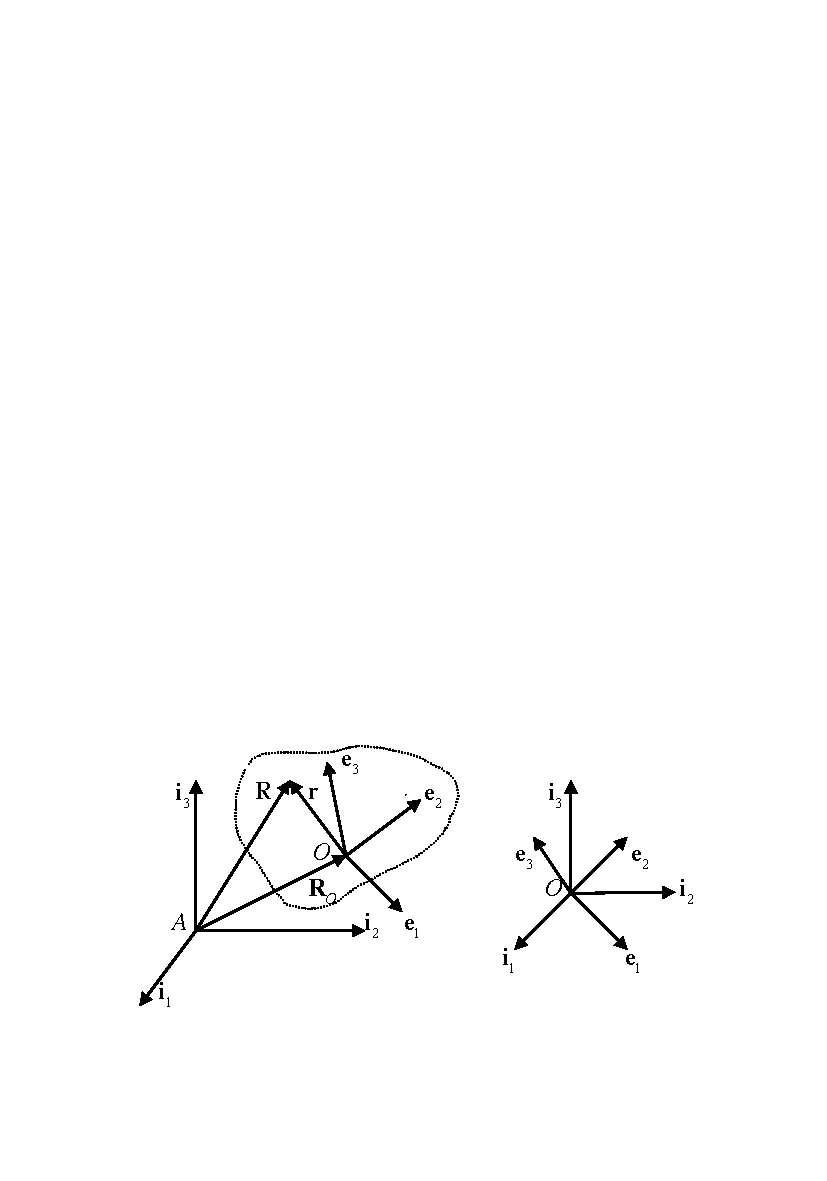
\includegraphics[width=0.8\textwidth]{pic/BI_notations.pdf}
\end{center}
Вращение твердого тела с неподвижной точкой задается нормированным
кватернионом $\mathbf{\Lambda}$ по формулам
$$
\mathbf{e}_k =
\mathbf{\Lambda}\circ\mathbf{i}_k\circ\overline{\mathbf{\Lambda}},
$$
каждому положению тела соответствуют два кватерниона, отличающихся знаком и
описывает преобразование $r_B\rightarrow r_I$.
\end{frame}
%--------------------------------------------------------------------------------
\begin{frame}
\frametitle{Способ определения поворота тела. Док-во (1/3)}
Получим выражение для искомого кватерниона в явном виде. Для этого введем
обозначения
$$
\mathbf{r}_k = \mathbf{e}_k - \mathbf{i}_k,\quad \mathbf{s}_k = \mathbf{e}_k +
\mathbf{i}_k ;\quad k=1, 2, 3.
$$
Для этих векторов выполнены следующие соотношения:
$$
\mathbf{s}_k\cdot\mathbf{r}_k = 0, \quad \mathbf{s}_j\cdot\mathbf{r}_k =
-\mathbf{s}_k\cdot\mathbf{r}_j
$$
\end{frame}
%--------------------------------------------------------------------------------
\begin{frame}
\frametitle{Способ определения поворота тела. Док-во (2/3)}    
Запишем теперь уравнения для искомого кватерниона в следующем виде (домножив
исходные уравнения на кватернион $\mathbf{\Lambda}$ справа:
$$
\mathbf{e}_k\circ\mathbf{\Lambda} = \mathbf{\Lambda}\circ\mathbf{i}_k,
$$
что можно переписать в виде следующей системы:
$$
\left\{
\begin{array}{l}
    \mathbf{e}_k\cdot\mathbf{\lambda} = \mathbf{i}_k\cdot\mathbf{\lambda} \\
    \lambda_0\mathbf{e}_k + \mathbf{e}_k\times\mathbf{\lambda} =
    \lambda_0\mathbf{i}_k - \mathbf{i}_k\times\mathbf{\lambda}
\end{array}
\right. \Rightarrow
\left\{
\begin{array}{l}
    \mathbf{r}_k\cdot\mathbf{\lambda} = 0 \\
    \lambda_0\mathbf{r_k} = \mathbf{\lambda}\times\mathbf{s}_k
\end{array}
\right. .
$$
В случае, если базисы совпадают, решение $\lambda_0=\pm 1$ очевидно. Пусть в
общем случае векторы $\mathbf{r}_1$ и $\mathbf{r}_2$ не равны нулю. Тогда
векторная часть искомого решения может быть записана в виде $\mathbf{\lambda}
= x\left(\mathbf{r}_1\times\mathbf{r}_2\right)$, где $x$ -- некоторый скаляр.
\end{frame}
%--------------------------------------------------------------------------------
\begin{frame}
\frametitle{Способ определения поворота тела. Док-во (3/3)}    
Подставляя полученное выражение во второе уравнение системы, получаем, что
$$
\left\{
\begin{array}{l}
    \lambda_0\mathbf{r}_1 =
    -x\mathbf{s}_1\times\left(\mathbf{r}_1\times\mathbf{r}_2\right)
    =-x\mathbf{r}_1\left(\mathbf{s}_1\cdot\mathbf{r}_2\right)\\
    \lambda_0\mathbf{r}_2 =
    -x\mathbf{s}_2\times\left(\mathbf{r}_1\times\mathbf{r}_2\right)
    =-x\mathbf{r}_2\left(\mathbf{s}_2\cdot\mathbf{r}_1\right)\\
\end{array}
\right. .
$$
Оба полученных уравнение тождественно равны, потому
$$
\mathbf{\Lambda} = x\left(\mathbf{s}_2\cdot\mathbf{r}_1 +
\mathbf{r}_1\times\mathbf{r}_2\right)
$$
Теорема Эйлера о вращении твердого тела следует непосредственно из приведения
кватерниона к тригонометрическому виду
$$
\mathbf{\Lambda}=\left(\cos{\phi}+\mathbf{e}\sin{\phi}\right)
$$
\begin{itemize}
\item Вращение тела осуществляется вдоль оси, направление которой совпадает с
    векторной частью кватерниона
\item Угол поворота составляет $2\phi$.
\end{itemize}
\end{frame}
%--------------------------------------------------------------------------------
\begin{frame}
\frametitle{Кватернионное сложение поворотов}
Пусть $\mathbf{\Lambda}$ задает поворот из
базиса $\mathbf{I}$ в базис $\mathbf{I}'$, а кватернион $\mathbf{M}$ -- из
базиса $\mathbf{I}'$ в базис $\mathbf{I}''$. Тогда начальное положение точки
$\mathbf{r}$ преобразуется в конечное положение точки $\mathbf{r}''$ в соответствии с
преобразованием
$$
\mathbf{r}'' = \mathbf{M}\circ\mathbf{r}'\circ\overline{\mathbf{M}} =
\mathbf{M}\circ\mathbf{\Lambda}\circ\mathbf{r}\circ\overline{\mathbf{\Lambda}}\circ\overline{\mathbf{M}}
= \mathbf{N}\circ\mathbf{r}\circ\overline{\mathbf{N}}, \quad \mathbf{N} =
\mathbf{M}\circ\mathbf{\Lambda}
$$
\begin{center}
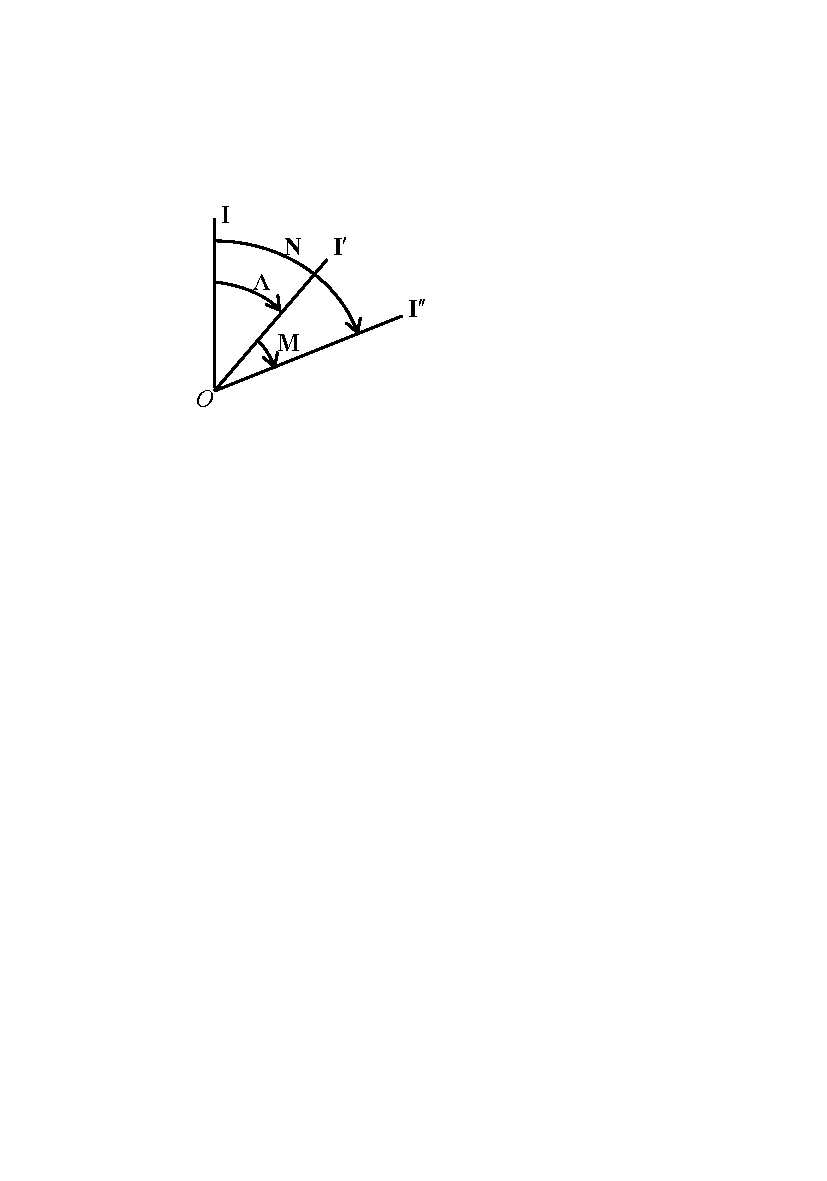
\includegraphics[width=0.4\textwidth]{pic/multiple_rotations.pdf}
\end{center}
\end{frame}
%--------------------------------------------------------------------------------
\section{Кинематические уравнения Эйлера}
%--------------------------------------------------------------------------------
\begin{frame}
\frametitle{Динамика кватерниона}
Для написания уравнений движения твердого тела и дальнейшей фильтрации
наблюдений необходимо записать уравнение производной для кватерниона, а затем
эти уравнения линеаризовать. Динамика кватерниона задается уравнением
Пуассона. Угловая скорость в базисе $\mathbf{I}$ -- это
$$
\mathbf{\omega}=\lim_{\Delta t \rightarrow 0}\frac{\Delta\phi\left(t,\Delta t\right)}{\Delta
t}\mathbf{e}\left(t,\Delta t\right)
$$
Изменению поворота соответствует следующее изменение кватерниона
$$
\delta\mathbf{\Lambda}=\cos{\frac{\Delta\phi\left(t,\Delta t\right)}{2}} + \mathbf{e}\left(t,\Delta t\right)
\sin{\frac{\Delta\phi\left(t,\Delta t\right)}{2}} =
$$
$$
= 1 + \mathbf{e}\left(t,\Delta t\right)
{\frac{\Delta\phi\left(t,\Delta t\right)}{2}} + O\left(\left(\Delta\phi\right)^2\right)
$$
Этот кватернион определяется из формулы сложения поворотов:
$$
\mathbf{\Lambda}\left(t+\Delta t\right) = \delta \mathbf{\Lambda} \circ
\mathbf{\Lambda}\left(t\right)
$$
\end{frame}
%--------------------------------------------------------------------------------
\begin{frame}
\frametitle{Уравнение Пуассона}
$$
\mathbf{\Lambda}\left(t+\Delta t\right) - \mathbf{\Lambda}\left(t\right)
=\delta \mathbf{\Lambda}\circ\mathbf{\Lambda}\left(t\right)
-\mathbf{\Lambda}\left(t\right) \Rightarrow \Delta \mathbf{\Lambda} =
\left(\delta \mathbf{\Lambda}-1\right)\circ \mathbf{\Lambda}\left(t\right)
$$
Вычисляя предел при $\Delta t \rightarrow 0$, получаем следующие соотношения:
$$
\dot{\mathbf{\Lambda}} = \lim_{\Delta t \rightarrow 0}{\frac{\Delta
\mathbf{\Lambda}}{\Delta t}} =  \lim_{\Delta t \rightarrow 0}{\frac{\delta
\mathbf{\Lambda}}{\Delta t}}\circ \mathbf{\Lambda}\left( t \right) =
\frac{1}{2}\mathbf{\omega}_I\circ\mathbf{\Lambda}.
$$
Для сравнения с углами Эйлера:
\begin{center}
    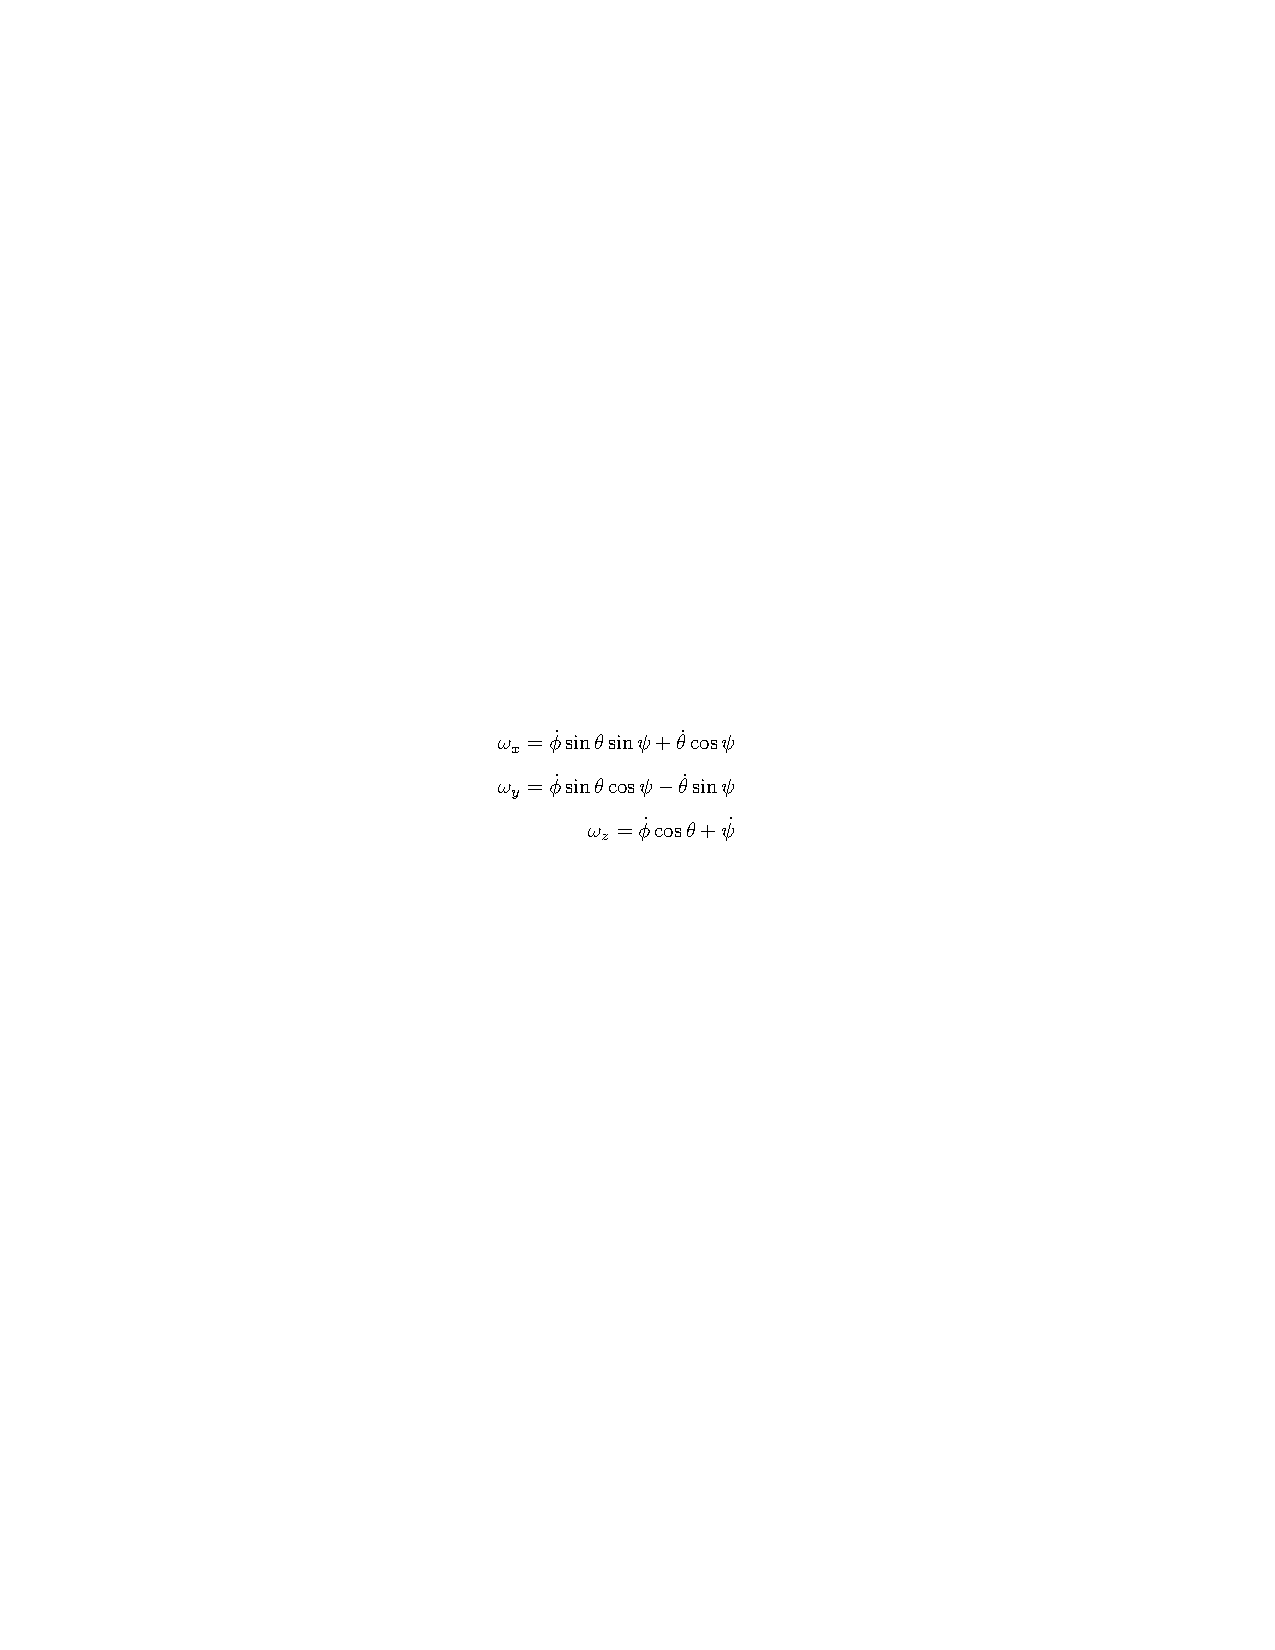
\includegraphics[width=0.5\textwidth]{pic/euler_dot.pdf}
\end{center}
\end{frame}
%--------------------------------------------------------------------------------
\begin{frame}
\frametitle{Уравнение Пуассона}
$$
\dot{\mathbf{\Lambda}} =
\frac{1}{2}\mathbf{\omega}_I\circ\mathbf{\Lambda}.
$$
Полученные уравнения являются являются кинематическими уравнениями
вращательного движения твердого тела, записанными в кватернионах, и называются
уравнениями Пуассона -- четыре скалярных дифференциальных уравнения, которые
связывают параметры Родрига-Гамильтона с проекциями угловой скорости тела
на оси базиса $\mathbf{I}$ -- инерциальной системы отсчета.

В некоторых ситуациях угловая скорость задается в проекциях на оси базиса,
связанного с телом. В этом случае
$$
\mathbf{\omega}_I =
\mathbf{\Lambda}\circ\mathbf{\omega}_B\circ\overline{\mathbf{\Lambda}}.
$$
Тогда уравнение Пуассона имеет иной вид:
$$
\dot{\mathbf{\Lambda}} = \frac{1}{2}\mathbf{\Lambda}\circ\mathbf{\omega}_B.
$$
\end{frame}
%--------------------------------------------------------------------------------
\section{Расширенный фильтр Калмана. }
%--------------------------------------------------------------------------------
\begin{frame}
\frametitle{Оцениваемый фазовый вектор}

\begin{itemize}
\item[$q_{BI}$] кватернион, задающий ориентацию тела -- векторная его часть,
    скалярная может быть вычислена исходя из единичной нормы кватерниона;
\item[$\omega_B$] вектор угловой скорости, заданный в проекциях на \emph{собственные
    оси} твердого тела с \emph{добавленным смещением показаний гироскопа}
\item[$\omega_{I}^{bias}$] смещение показаний гироскопа, выраженное в
    проекциях на \emph{инерциальные} оси.
\end{itemize}
Угловая скорость выражена в собственных осях
\begin{enumerate}
    \item Оценка угла поворота колес задает соответствие между линейной
        скоростью движения и угловой скоростью в собственных осях
    \item Разность ускорений, измеренных в точке центра масс и в любой другой
        точке твердого тела, определяется из соотношения угловых скоростей,
        выраженных в собственных осях и геометрией расположения
        акселерометров.
\end{enumerate}
\end{frame}
%--------------------------------------------------------------------------------
\begin{frame}
\frametitle{Почему с ``добавленным смещением показаний гироскопа''?}
Рассмотрим линейный одномерный случай прямолинейного движения с изменением
координаты и скорости со смещением. Предиктор:
$$
\rho_{k+1|k} = \mathbf{F}\rho_{k_k}, \quad \rho = \left(x, v,
v^{bias}\right)^T.
$$
$$
\mathbf{P}_{k+1|k} = \mathbf{FP}_{k|k}\mathbf{F}^T + \mathbf{Q}\left(\Delta
t\right),\quad
\mathbf{F} = \mathbf{E}_{3\times 3} + \left(\begin{array}{ccc}
0 & 1 & -1 \\
0 & 0 & 0 \\
0 & 0 & 0
\end{array}\right)\Delta t
$$
Наблюдение координаты и скорости:
$$
\mathbf{H}_x = \left(\begin{array}{ccc} 1 & 0 & 0\end{array}\right),\quad
\mathbf{H}_v = \left(\begin{array}{ccc} 0 & 1 & 0\end{array}\right)
$$
Шаг корректора
$$
\mathbf{S} = \mathbf{HP}_{k|k+1}
\mathbf{H}^T + \mathbf{R},\quad
\mathbf{K} = \mathbf{P}_{k|k+1}
\mathbf{H}^T\mathbf{S}^{-1},\quad
\mathbf{P}_{k+1|k+1} = 
\left(\mathbf{E}-\mathbf{KH}\right)\mathbf{P}_{k|k+1}
$$
\end{frame}
%--------------------------------------------------------------------------------
\section{Линеаризация кинематических уравнений}
%--------------------------------------------------------------------------------
\begin{frame}
\frametitle{Линеаризация уравнений динамики}
Имеем фазовый вектор
$$
\rho = \left(q_{BI}, \omega_B, \omega_I^{bias}\right)^T
$$
В силу единичной нормы кватерниона, в фазовый вектор входит только его
векторная часть. Линеаризованная динамика этого вектора подчиняется уравнению
$$
\dot{\rho}\left(t\right) = \mathbf{F}\left(t, \rho\right)\rho
$$
Рассмотрим малое возмущение фазового вектора $\rho = \hat{\rho} + \delta\rho$,
тогда
$$
\frac{d\hat{\rho}\left(t\right)}{dt} = \mathbf{F}\left(t, \rho\right)\hat{\rho},\quad
\frac{d\delta{\rho}\left(t\right)}{dt} = \mathbf{F}\left(t, \rho\right)\delta{\rho}
$$
Под приращением кватерниона будем понимать малый поворот:
$$
\hat{q}_{k+1} = \delta q \circ \hat{q}_{k}
$$
Такая замена традиционного приращения позволит существенно упростить вид
уравнений фильтра.
\end{frame}
%--------------------------------------------------------------------------------
\begin{frame}
\frametitle{Линеаризация уравнения Пуассона}
Линеаризованный вид динамики вращения следует напрямую из уравнения Пуассона:
$$
\dot{\mathbf{\Lambda}} =
\frac{1}{2}\mathbf{\Lambda}\circ\mathbf{\omega}_B,\quad
\dot{\mathbf{\Lambda}} = \frac{1}{2}\mathbf{\omega}_I\circ\mathbf{\Lambda}.
$$
Первые три ряда матрицы $\mathbf{F}$
$$
\left(\begin{array}{ccc}
        \mathbf{0}_{3\times 3} & \frac{1}{2}\mathbf{A}^T &
        -\frac{1}{2}\mathbf{E}_{3\times 3}
\end{array}\right),
$$
остальные элементы матрицы равны нулю.  Матрица $\mathbf{A}$ задает следующее
линейное  преобразование:
$$
\mathbf{\omega}_B = \mathbf{A}\mathbf{\omega}_I, 
$$
Скалярная часть приращения кватерниона равна единице, что потребует
перенормировки кватерниона на каждом шаге работы фильтра.
\end{frame}
%--------------------------------------------------------------------------------
\begin{frame}
    \frametitle{Линеаризация наблюдений гироскопа (1/4)}
Линейная функция наблюдений задается следующими условиями:
$$
z = \mathbf{H}\rho \Rightarrow \delta z = \mathbf{H}\delta\rho.
$$
Получим линеаризованную функцию наблюдений гироскопа. Линеаризуем соотношение
$$
\hat{\mathbf{\omega}}_{meas} = \mathbf{A}^T\hat{\mathbf{\omega}_B}.
$$
где матрица $ \mathbf{A}$ задает преобразование $\mathbf{\omega}_B =
\mathbf{A}\mathbf{\omega}_I$. Истинное ожидаемое наблюдение представляет собой
оценку ожидаемого наблюдения с некоторым (малым) возмущением)
$$
\mathbf{\omega}_m = \hat{\mathbf{\omega}} + \delta\mathbf{\omega}
$$
\end{frame}
%--------------------------------------------------------------------------------
\begin{frame}
    \frametitle{Линеаризация наблюдений гироскопа (2/4)}
Для начала перепишем уравнение Пуассона в матричном виде, обозначив отдельно
скалярную и векторную части кватерниона
$$
\left(
\begin{array}{c}
    \dot{q}_0 \\
    \dot{\mathbf{q}}
\end{array}
\right) = \frac{1}{2}\mathbf{C}
\left(
\begin{array}{c}
    {q}_0 \\
    {\mathbf{q}}
\end{array}
\right),
\quad
\mathbf{C} = \left(\begin{array}{cc}
0 & -\mathbf{\omega}^T \\
\mathbf{\omega} & \mathbf{W} 
\end{array}\right)
$$
$$
\mathbf{W} = \left(\begin{array}{rrr}
        0 & \omega_3 & -\omega_2 \\
        -\omega_3 & 0 & \omega_1 \\
        \omega_2 & -\omega_1 & 0
\end{array}\right)
$$
Вектор угловой скорости записан в собственных осях
\end{frame}
%--------------------------------------------------------------------------------
\begin{frame}
    \frametitle{Линеаризация наблюдений гироскопа (3/4)}
С учетом того, что
$$
\mathbf{A}\left(\delta q \circ q\right) =
\mathbf{A}\left(q\right)\mathbf{A}\left(\delta q\right), \quad
\mathbf{A}^T\left(\delta q \circ q\right) =
\mathbf{A}^T\left(\delta q\right)\mathbf{A}^T\left(q\right),
$$
а матрица поворота, определяемая малым кватернионом (т. е. кватернионом с
малой векторной частью), имеет вид
$$
\mathbf{A}\left(\delta q\right) = \mathbf{E} + 2\mathbf{W}_{\delta q},\quad
\mathbf{A}^T\left(\delta q\right) = \mathbf{E} - 2\mathbf{W}_{\delta q},
$$
где $\mathbf{W}_{\delta q}$ -- матрица косо-симметричного оператора, взятого со
знаком минус (аналогично $\mathbf{W}$). Тогда легко получить, что 
$$
\hat{\mathbf{\omega}}_m +\delta \mathbf{\omega}_m = \mathbf{A}^T\left(\delta q \circ
\hat{q}\right)\left(\hat{\mathbf{\omega}}_B + \delta \mathbf{\omega}_B\right) = 
\left(\mathbf{E} - 2\mathbf{W}_{\delta q}\right)\mathbf{A}^T\left(\hat{q}\right)
\left(\hat{\mathbf{\omega}}_B + \delta\mathbf{\omega}_B\right),
$$
$$
\hat{\mathbf{\omega}}_m +\delta \mathbf{\omega}_m = 
-2\mathbf{W}_{\delta q}\mathbf{A}^T\left(\hat{q}\right)\hat{\mathbf{\omega}}_B + 
\mathbf{A}^T\left(\hat{q}\right)
\left(\hat{\mathbf{\omega}}_B + \delta\mathbf{\omega}_B\right),
$$
$$
\delta \mathbf{\omega}_m = 
-2\mathbf{W}_{\delta q}\mathbf{A}^T\left(\hat{q}\right)\hat{\mathbf{\omega}}_B + 
\mathbf{A}^T\left(\hat{q}\right)\delta\mathbf{\omega}_B = 
-2\mathbf{W}_{\delta q}\hat{\mathbf{\omega}}_I + 
\mathbf{A}^T\left(\hat{q}\right)\delta\mathbf{\omega}_B.
$$
\end{frame}
%--------------------------------------------------------------------------------
\begin{frame}
    \frametitle{Линеаризация наблюдений гироскопа (4/4)}
$$
\delta \mathbf{\omega}_m = 
-2\mathbf{W}_{\delta q}\hat{\mathbf{\omega}}_I + 
\mathbf{A}^T\left(\hat{q}\right)\delta\mathbf{\omega}_B
$$
С учетом свойств антикоммутативности векторного произведения
$$
\delta \mathbf{\omega}_m = 2\mathbf{W}_{\hat{\mathbf{\omega}}_I} \delta q+ 
\mathbf{A}^T\left(\hat{q}\right)\delta\mathbf{\omega}_B.
$$
\begin{block}{Матрица наблюдения показаний гироскопа}
$$
\mathbf{H} = \left(\begin{array}{ccc}
2\mathbf{W}_{\hat{\mathbf{\omega}}_I} &
\mathbf{A}^T\left(\hat{q}\right) &
\mathbf{0}_{3\times 3}
\end{array}\right)
$$
\end{block}
\end{frame}
%--------------------------------------------------------------------------------
\begin{frame}
\frametitle{Линеаризация показаний магнитометра}
Пусть в инерциальной системе отсчета имеется некоторое опорное направление,
задаваемое вектором $r_I$. Сенсоры на борту робота позволяют измерить
компоненты этого вектора в собственных осях, то есть компоненты вектора $r_B$.
$$
\mathbf{r}_m = \hat{\mathbf{r}}_B + \delta \mathbf{r} = \mathbf{A}\left(\delta
q\circ \hat{q}\right)\left(\hat{\mathbf{r}}_I + \delta \mathbf{r}_I\right) = 
\mathbf{A}\left(\hat{q}\right)
\left(\mathbf{E} + 2\mathbf{W}_{\delta q}\right)\left(\hat{\mathbf{r}}_I +
\delta \mathbf{r}_I\right),
$$
$$
\delta \mathbf{r} =
2\mathbf{A}\left(\hat{q}\right)\mathbf{W}_{\delta q}\hat{\mathbf{r}}_I = 
-2\mathbf{A}\left(\hat{q}\right)\mathbf{W}_{\hat{\mathbf{r}}_I}\delta q.
$$
\begin{block}{Матрица наблюдений опорного направления \emph{ранга 2}}
$$
\mathbf{H} = \left(\begin{array}{ccc}
-2\mathbf{A}\left(\hat{q}\right)\mathbf{W}_{\hat{\mathbf{r}}_I} &
\mathbf{0}_{3\times 3} &
\mathbf{0}_{3\times 3}
\end{array}\right)
$$
\end{block}
\end{frame}
%--------------------------------------------------------------------------------
\section{Валидация фильтра}
%--------------------------------------------------------------------------------
\begin{frame}
\frametitle{Валидация линеаризованного уравнения Пуассона (1/4)}
Модель в дискретном времени с постоянным шагом
\begin{center}
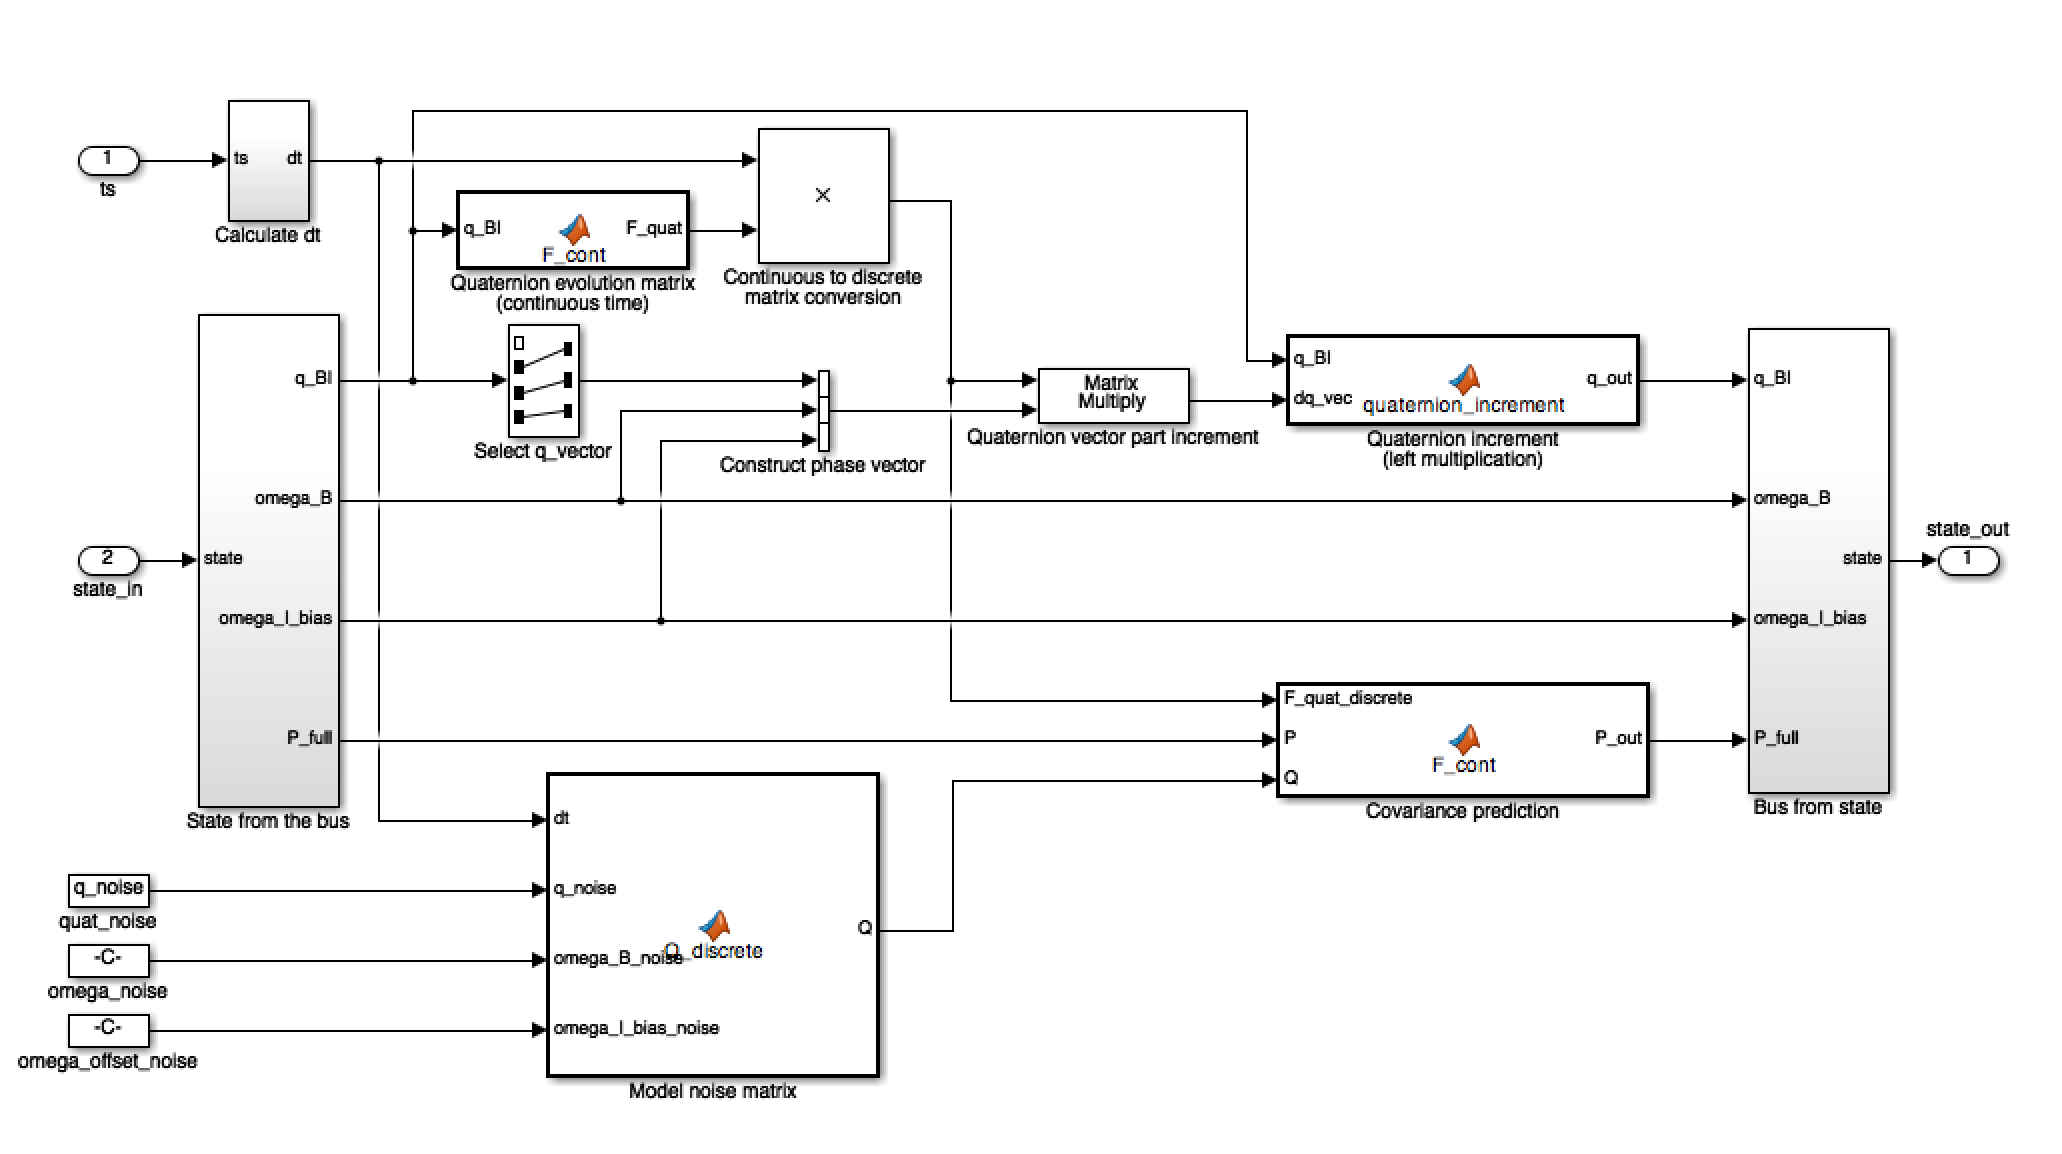
\includegraphics[width=\textwidth]{pic/kalman_predictor.png}
\end{center}
\end{frame}
%--------------------------------------------------------------------------------
\begin{frame}
\frametitle{Валидация линеаризованного уравнения Пуассона (2/4)}
Фазовые траектории для $\Delta t = 10^{-1}$ с.
\begin{center}
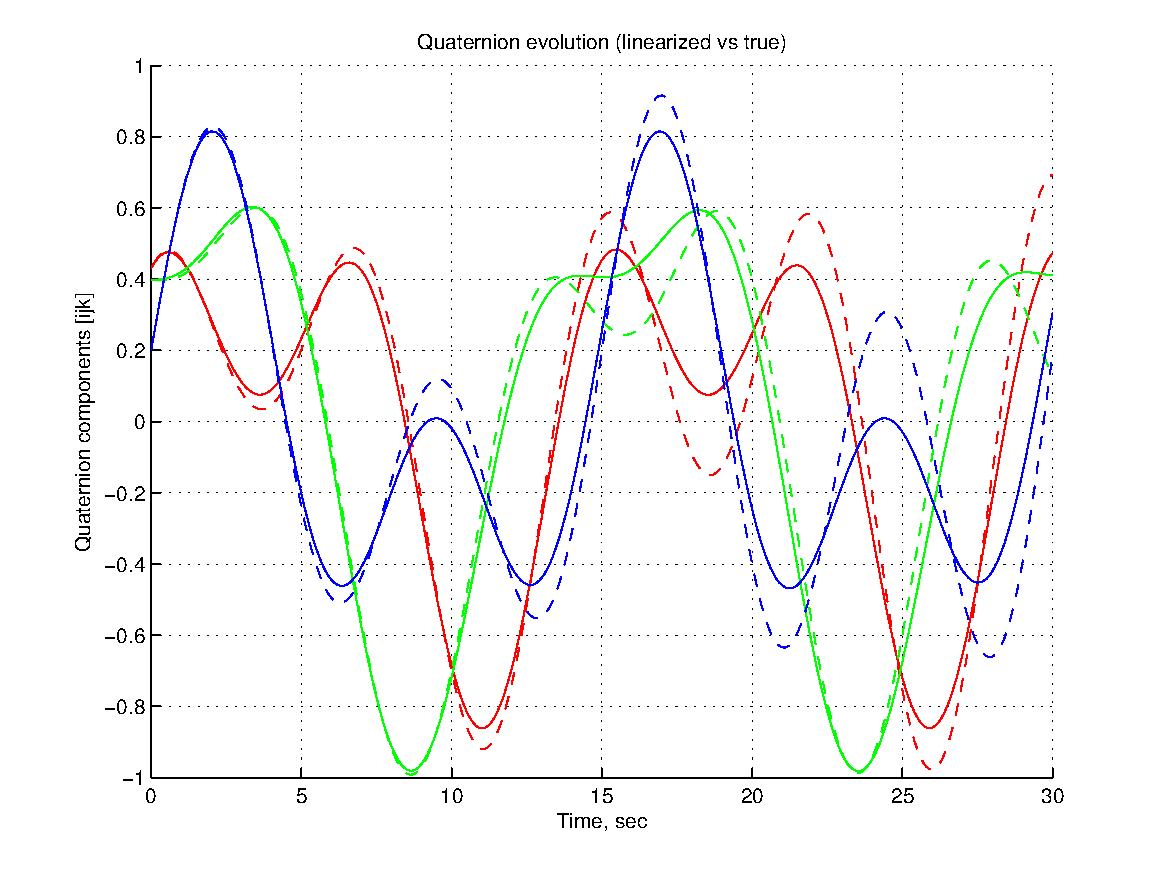
\includegraphics[width=0.8\textwidth]{pic/extrapolation_01.pdf}    
\end{center}
\end{frame}
%--------------------------------------------------------------------------------
\begin{frame}
\frametitle{Валидация линеаризованного уравнения Пуассона (3/4)}
Фазовые траектории для $\Delta t = 10^{-2}$ с.
\begin{center}
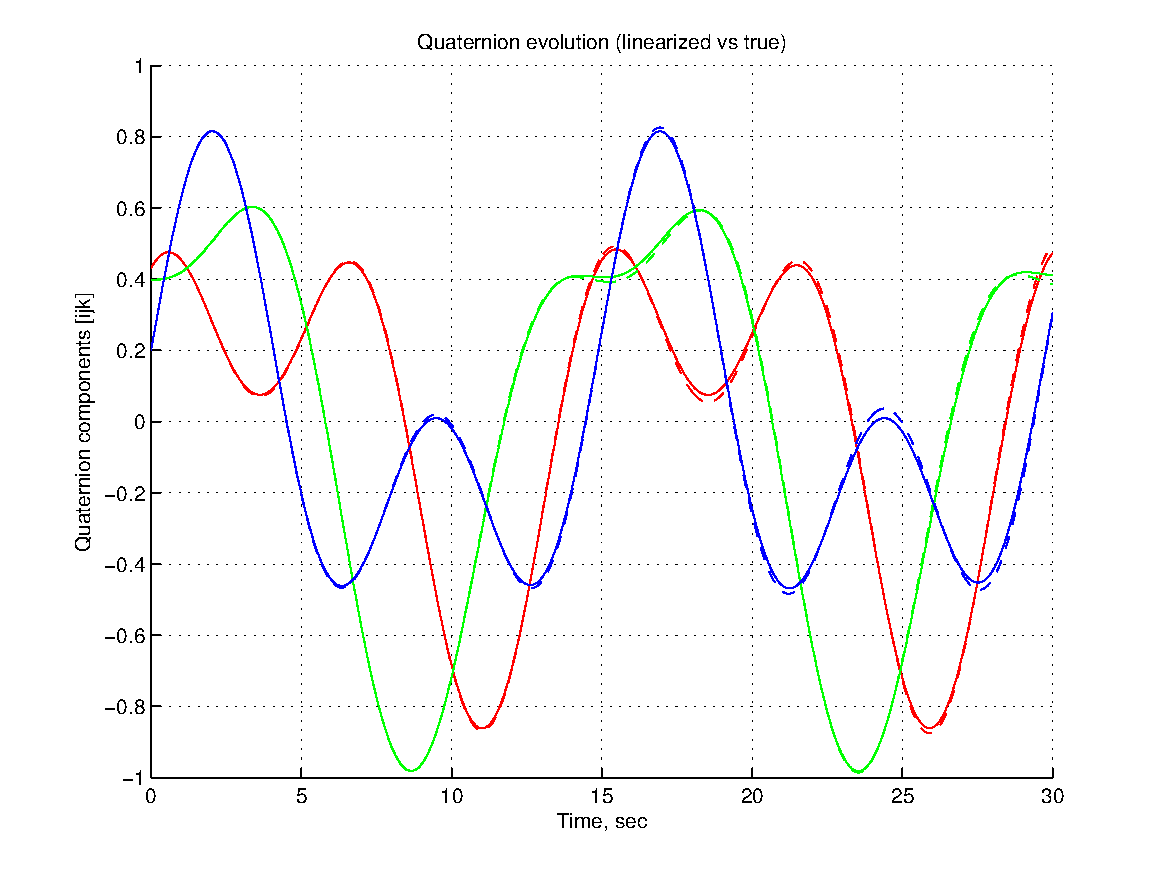
\includegraphics[width=0.8\textwidth]{pic/extrapolation_001.pdf}    
\end{center}
\end{frame}
%--------------------------------------------------------------------------------
\begin{frame}
\frametitle{Валидация линеаризованного уравнения Пуассона (4/4)}
Фазовые траектории для $\Delta t = 10^{-3}$ с.
\begin{center}
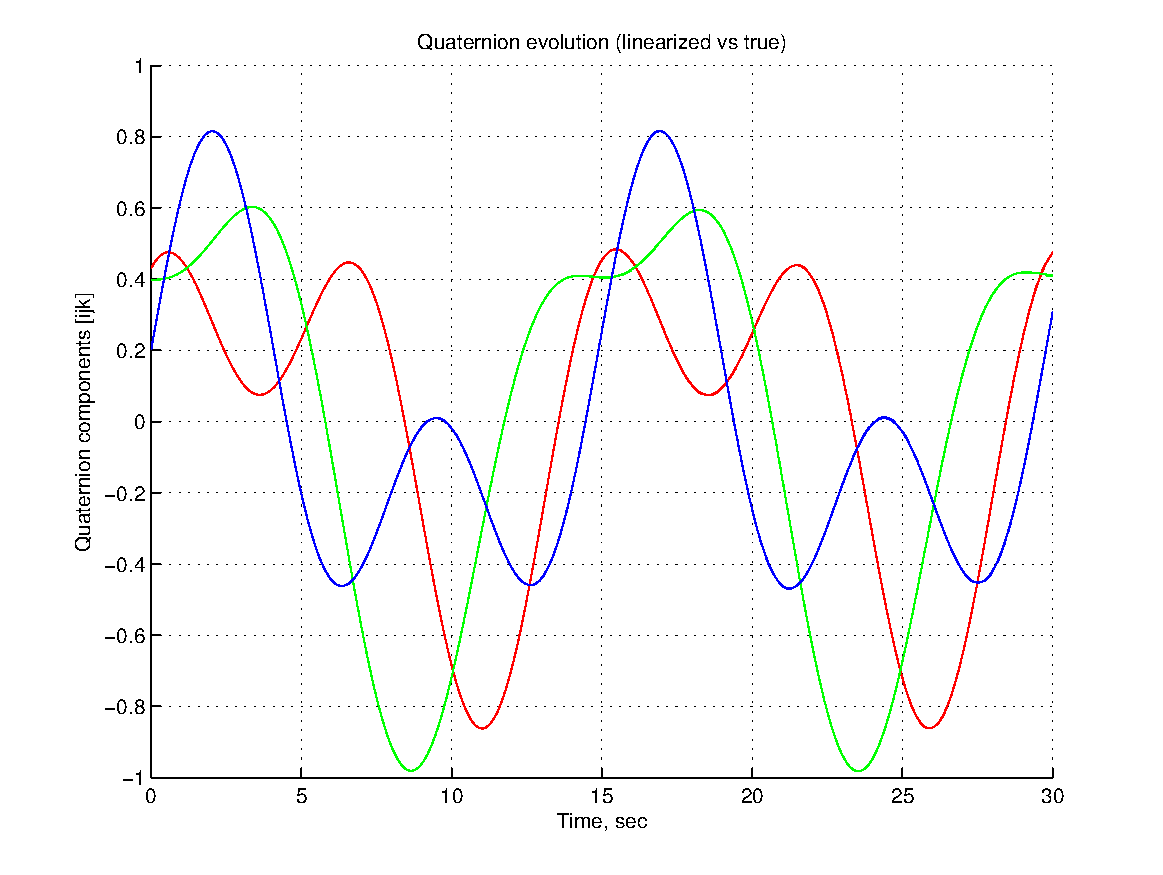
\includegraphics[width=0.8\textwidth]{pic/extrapolation_0001.pdf}    
\end{center}
\end{frame}
%--------------------------------------------------------------------------------
\begin{frame}
\frametitle{Валидация линеаризации наблюдений}
\begin{itemize}
    \item Выбрать опорные значения фазового вектора  -- случайные величины из
        распределения $\mathcal{N}\left(0, 1\right)$
    \item Выбрать малые приращения -- случайные величины из
        $\mathcal{N}\left(0, \frac{1}{N}\right)$, где $N$ -- варьируемый
        параметр
    \item Вычисление точного значения возмущенного наблюдения $\delta z$
    \item Вычисление линеаризованного возмущения $\delta z_{l}$
    \item Построение гистограммы величин
        $$
        \frac{\norm{\delta z - \delta z_l}}{\norm{\delta z}}
        $$
    \item Убедиться? что среднее значение полученной выборки равно
        $\frac{K}{N}$ для различных $N$, где $K$ -- постоянное число.
    \item Убедиться, что величина разброса существенно меньше одного порядка
\end{itemize}
\end{frame}
%--------------------------------------------------------------------------------
\begin{frame}
\frametitle{Валидация линеаризации наблюдения угловой скорости}
Гистограммы распределения 
$$
\frac{\norm{\delta z - \delta z_l}}{\norm{\delta z}}
$$
для $N = 100$ (слева) и $N=10$ (справа).
\begin{center}
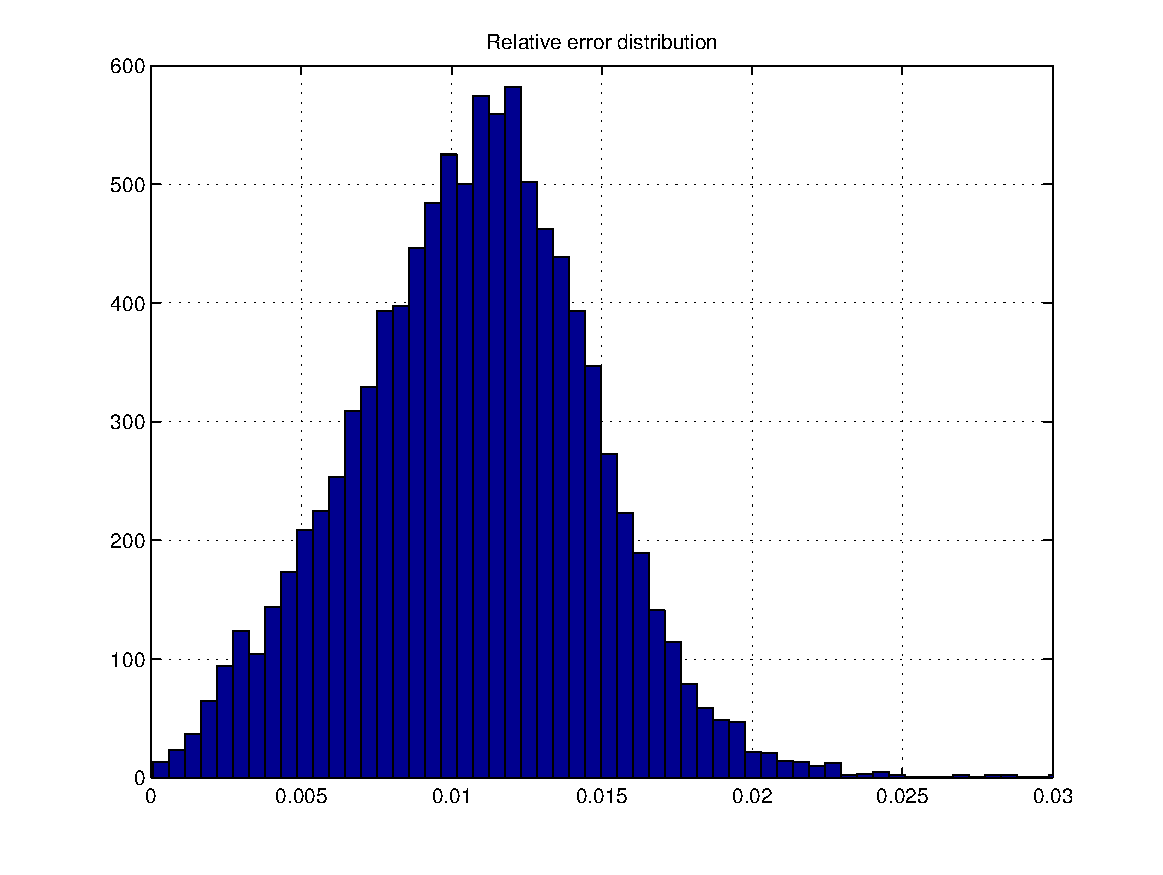
\includegraphics[width=0.4\textwidth]{pic/lin_gyro_001.pdf}    
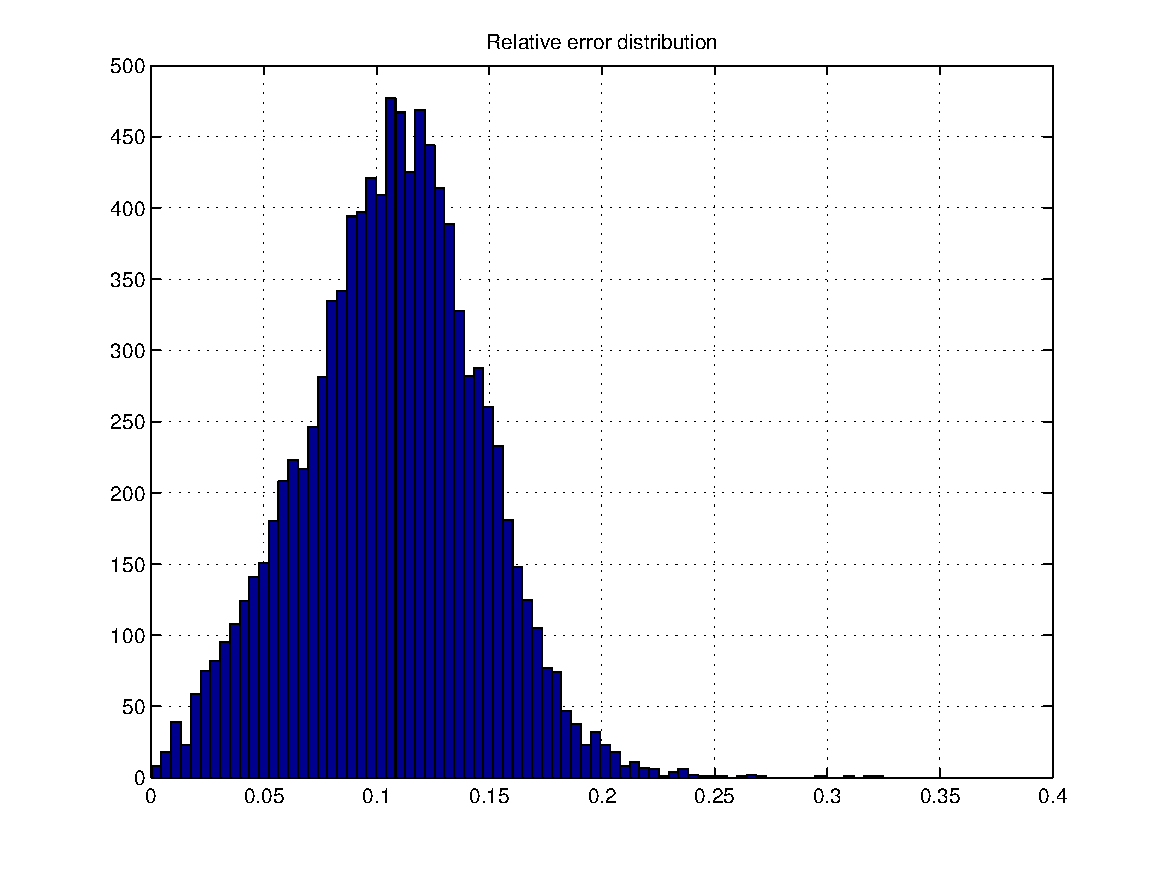
\includegraphics[width=0.4\textwidth]{pic/lin_gyro_01.pdf}    
\end{center}
\end{frame}
%--------------------------------------------------------------------------------
\begin{frame}
\frametitle{Валидация линеаризации наблюдения вектора магнитного поля}
Гистограммы распределения 
$$
\frac{\norm{\delta z - \delta z_l}}{\norm{\delta z}}
$$
для $N = 100$ (слева) и $N=10$ (справа).
\begin{center}
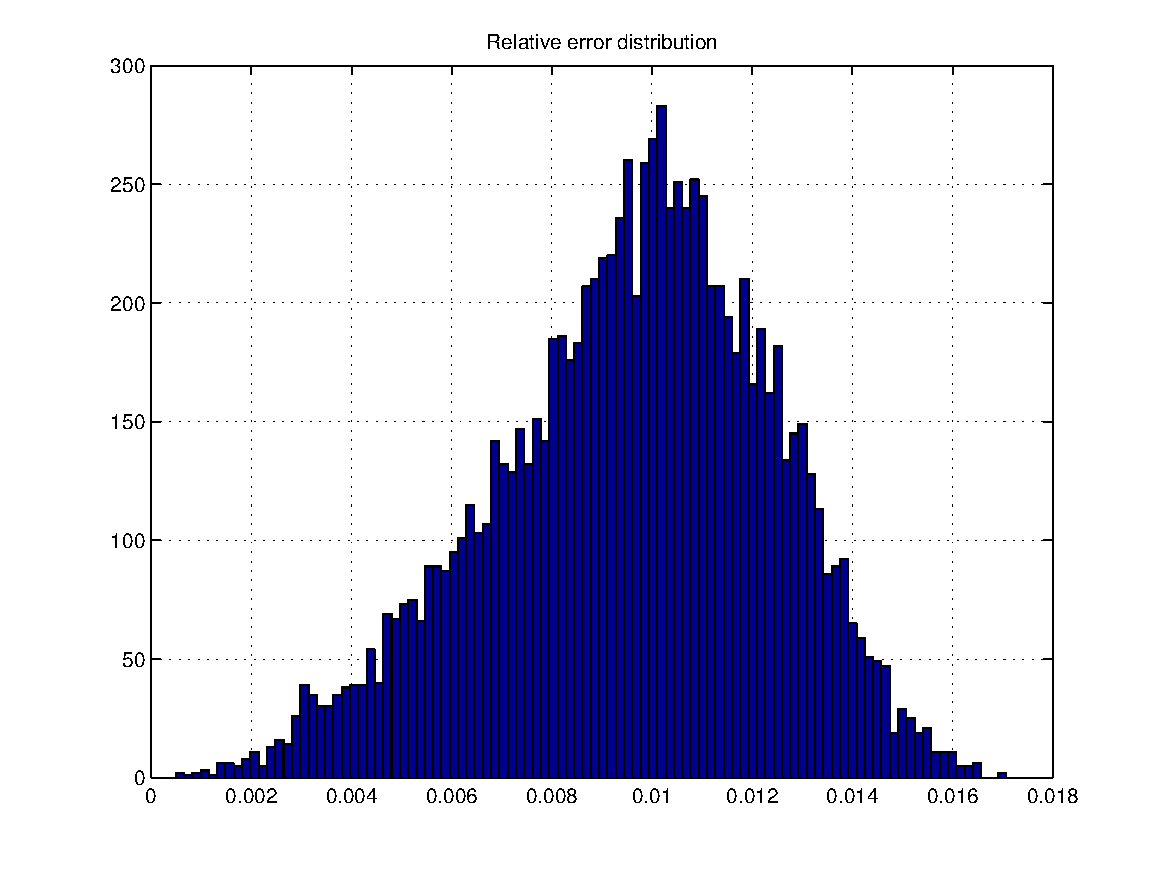
\includegraphics[width=0.4\textwidth]{pic/lin_direction_001.pdf}    
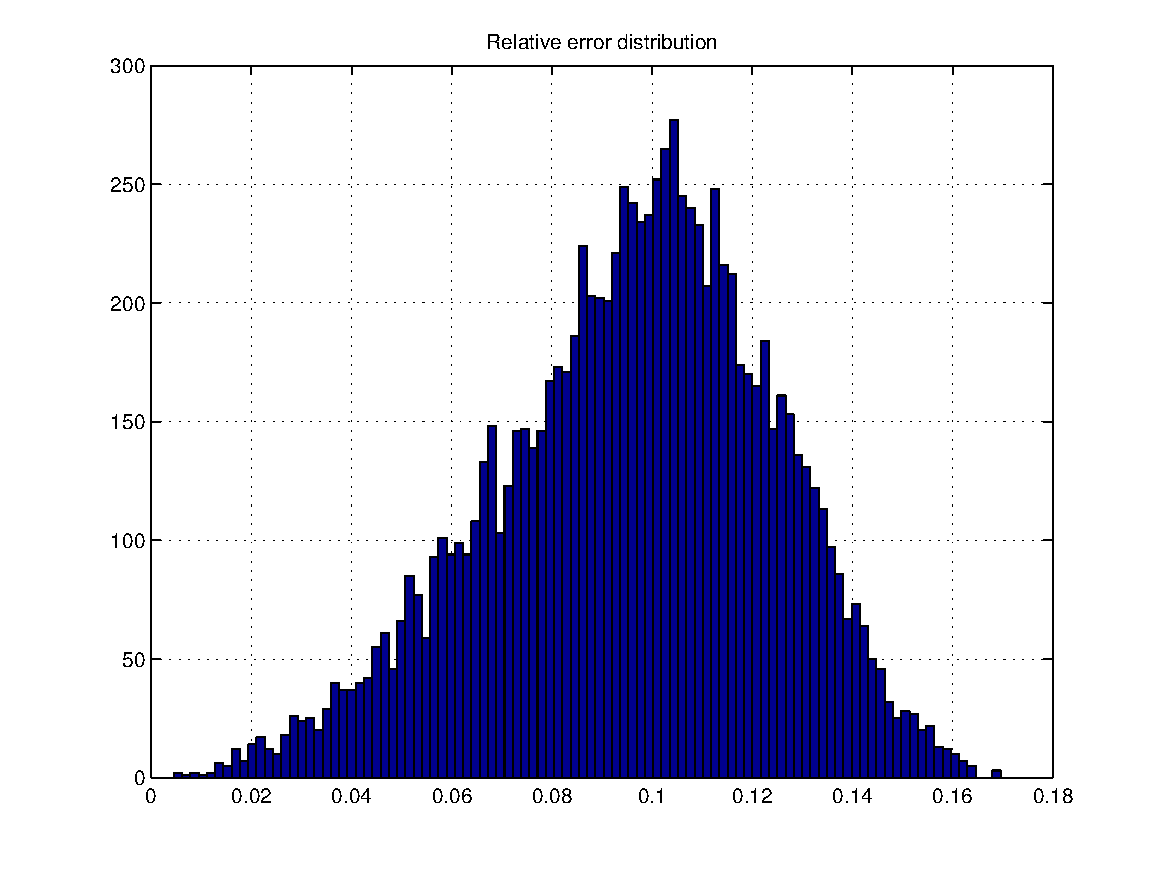
\includegraphics[width=0.4\textwidth]{pic/lin_direction_01.pdf}    
\end{center}
\end{frame}
%--------------------------------------------------------------------------------
\begin{frame}
\frametitle{Синхронный фильтр Калмана для двух опорных векторов и гироскопа (1/3)}
Модель в дискретном времени с постоянным шагом
\begin{center}
    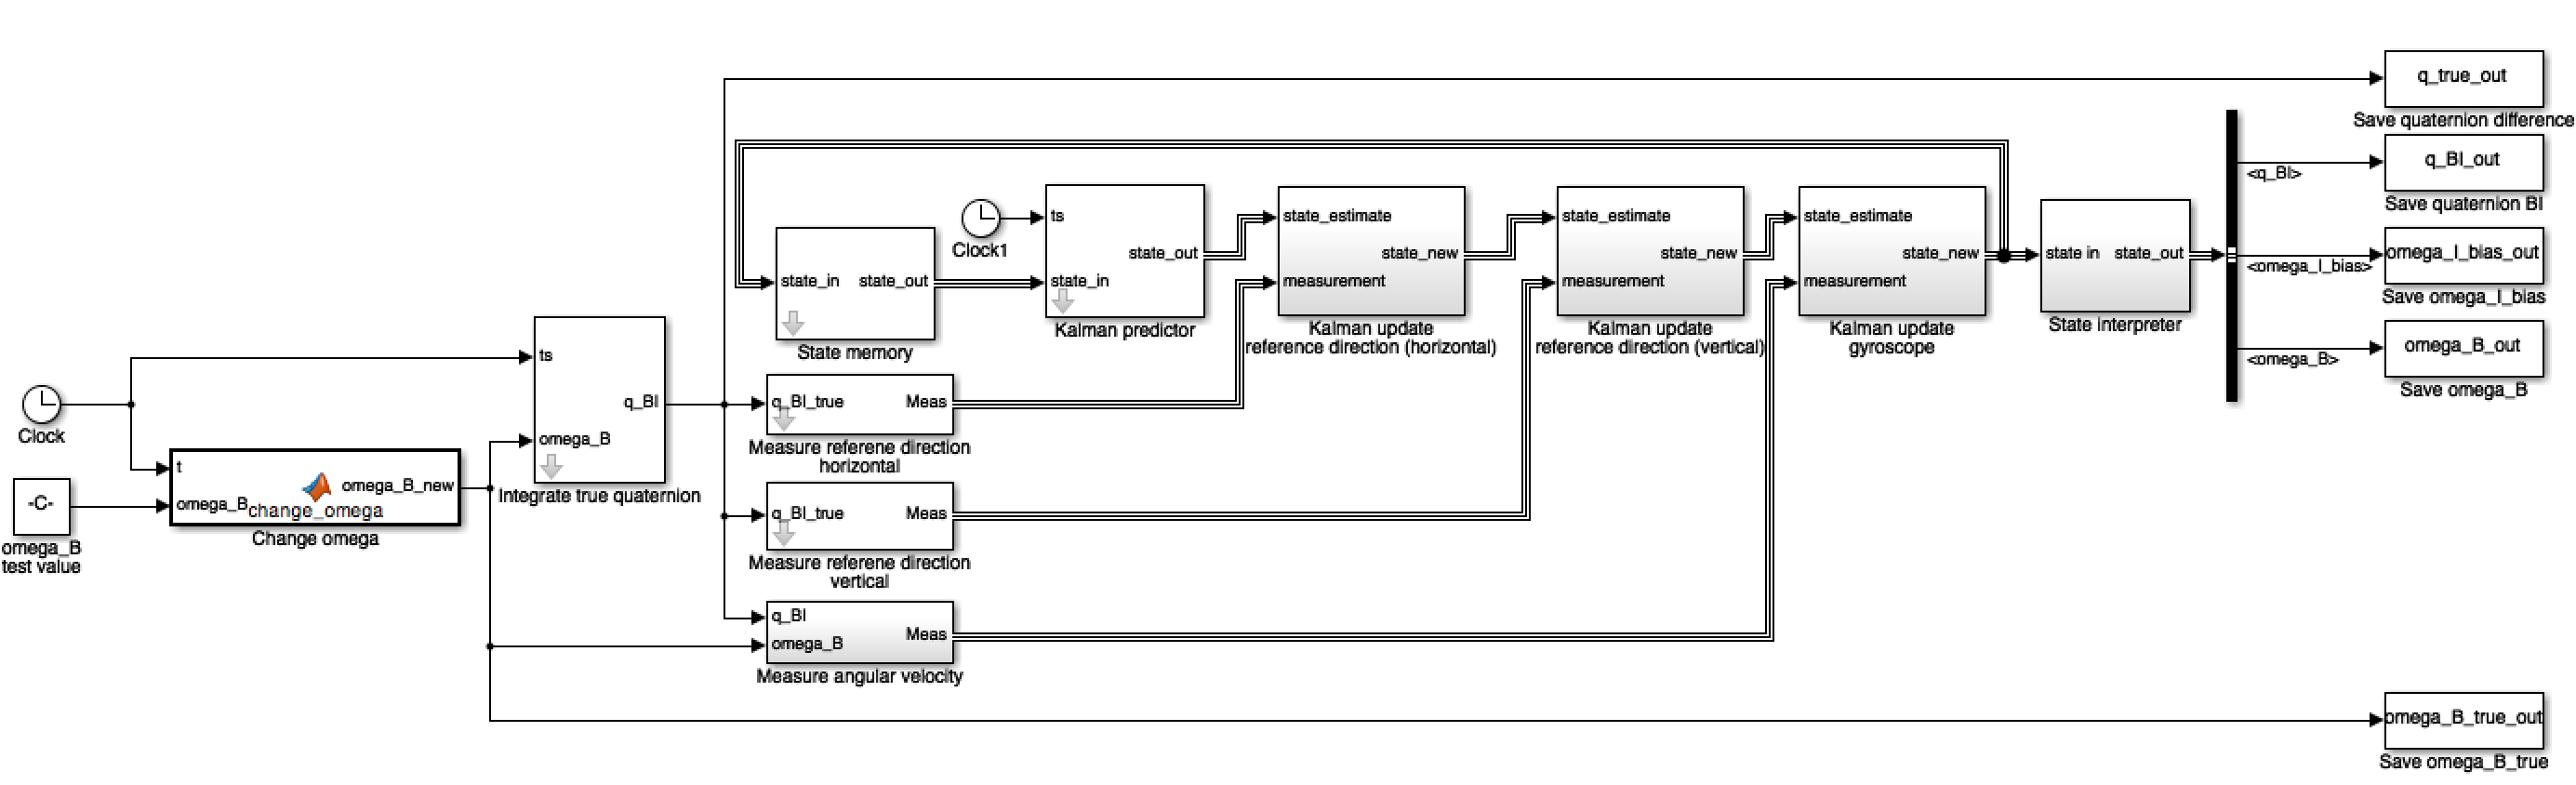
\includegraphics[width=\textwidth]{pic/kalman_gyro_sync.png}
\end{center}
\end{frame}
%--------------------------------------------------------------------------------
\begin{frame}
\frametitle{Синхронный фильтр Калмана для двух опорных векторов и гироскопа (2/3)}
\begin{center}
    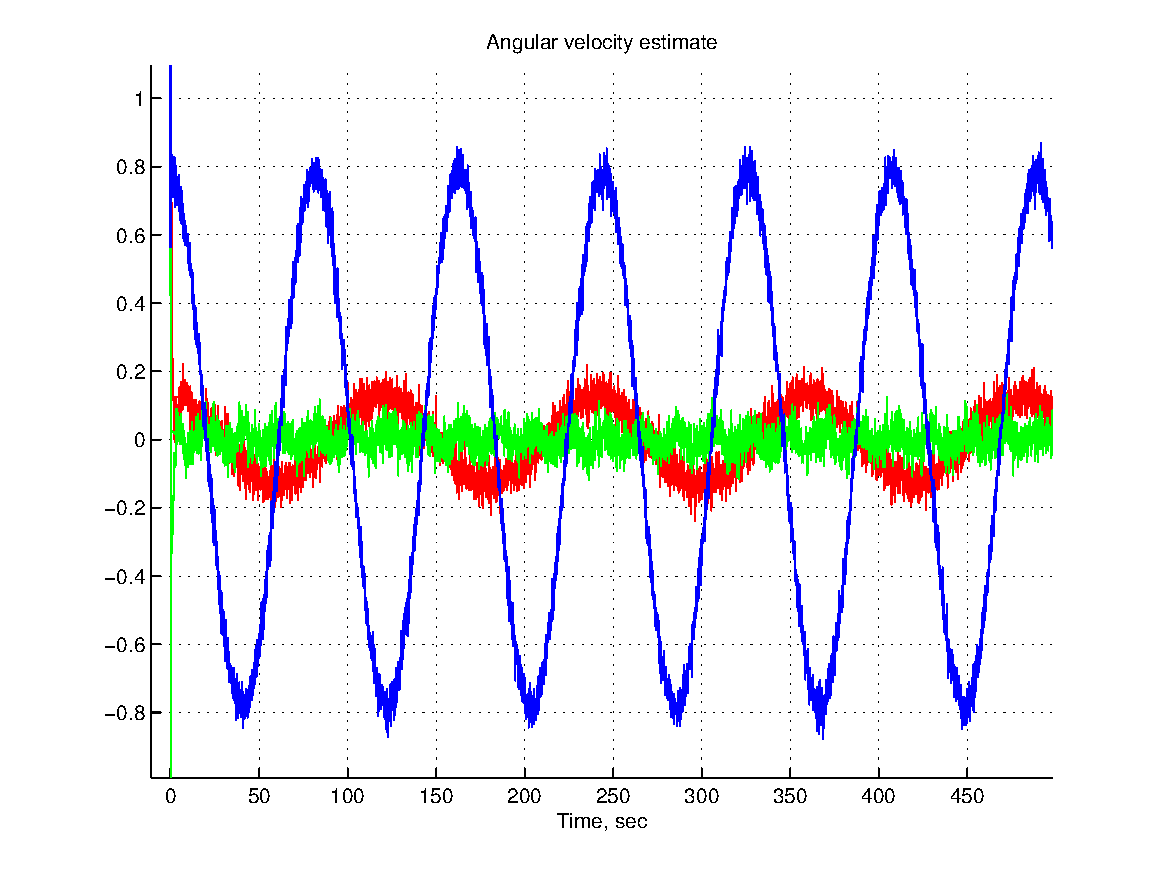
\includegraphics[width=0.8\textwidth]{pic/gyro_sync_omega.pdf}
\end{center}
\end{frame}
%--------------------------------------------------------------------------------
\begin{frame}
\frametitle{Синхронный фильтр Калмана для двух опорных векторов и гироскопа (3/3)}
\begin{center}
    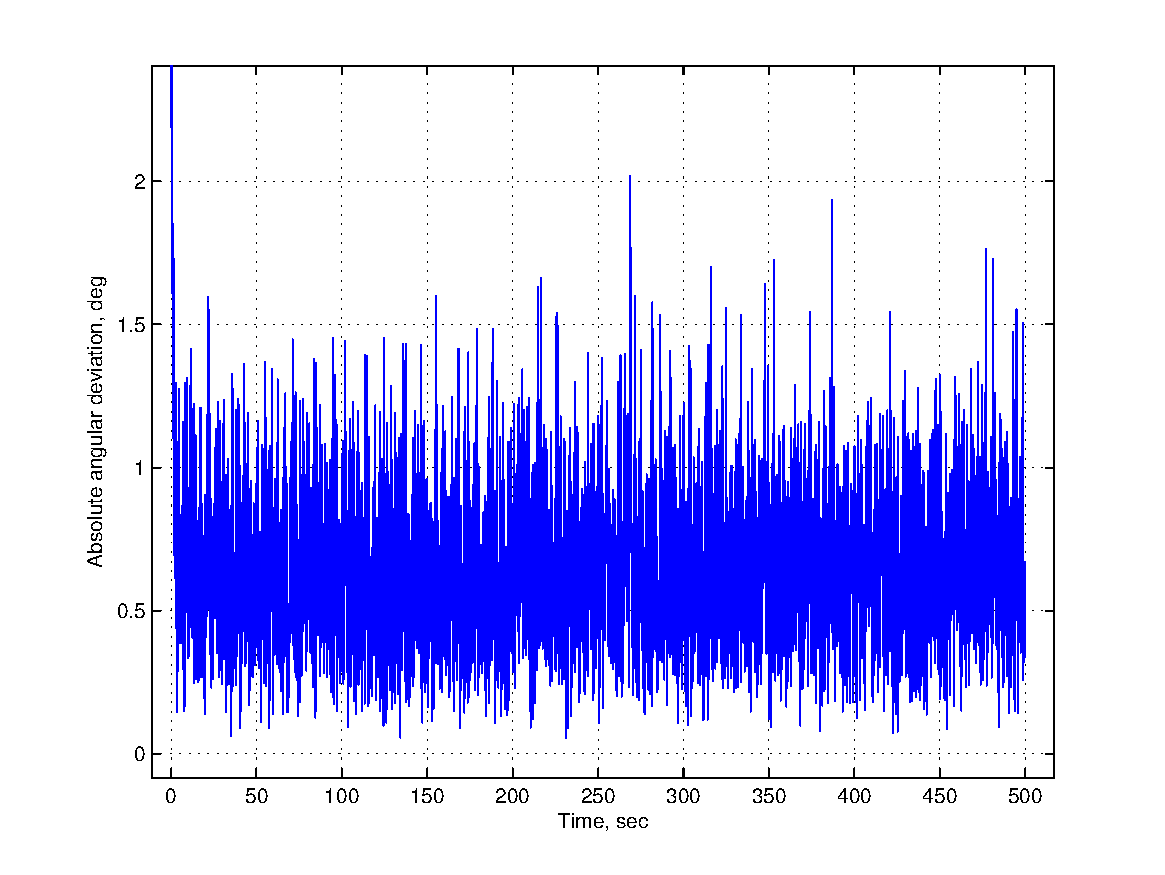
\includegraphics[width=0.8\textwidth]{pic/gyro_sync_dphi.pdf}
\end{center}
\end{frame}
%--------------------------------------------------------------------------------
\section{Наблюдаемость фазового вектора}
%--------------------------------------------------------------------------------
\begin{frame}
\frametitle{Уравнение Риккати для матрицы ковариации и наблюдаемость}
Динамика матрицы ковариации задается матричным уравнением Риккати
$$
\dot{\mathbf{P}}=\mathbf{Q} + \mathbf{F}\mathbf{P}+\mathbf{P}\mathbf{F}^T-\mathbf{P}\mathbf{H}^T
\mathbf{R}^{-1}\mathbf{H}\mathbf{P}^T
$$
Если максимальное собственное число убывает со временем -- тогда состояние
наблюдаемо. Доказано, что динамика \emph{матрицы Фишера} $\mathbf{I}$
расширенного фильтра Калмана подчиняется уравнению ($\mathbf{Q}\equiv0$ в этом
случае)
$$
\dot{\mathbf{I}} =
-\mathbf{F}^T\mathbf{I}-\mathbf{IF}+\mathbf{H}^T\mathbf{R}^{-1}\mathbf{H}
$$
Если ранг матрицы $\mathbf{I}$ вдоль некоторой траектории равен размерности
фазового вектора -- тогда состояние наблюдаемо.
При наблюдении единственного опорного вектора ранг матрицы наблюдений равен 5,
ранг матрицы информации Фишера не превышает 7 при $\omega_I\equiv const$.
\end{frame}
\begin{frame}
\frametitle{Валидация наблюдаемости состояния}
Непрерывное время, $ode45$.
\begin{center}
    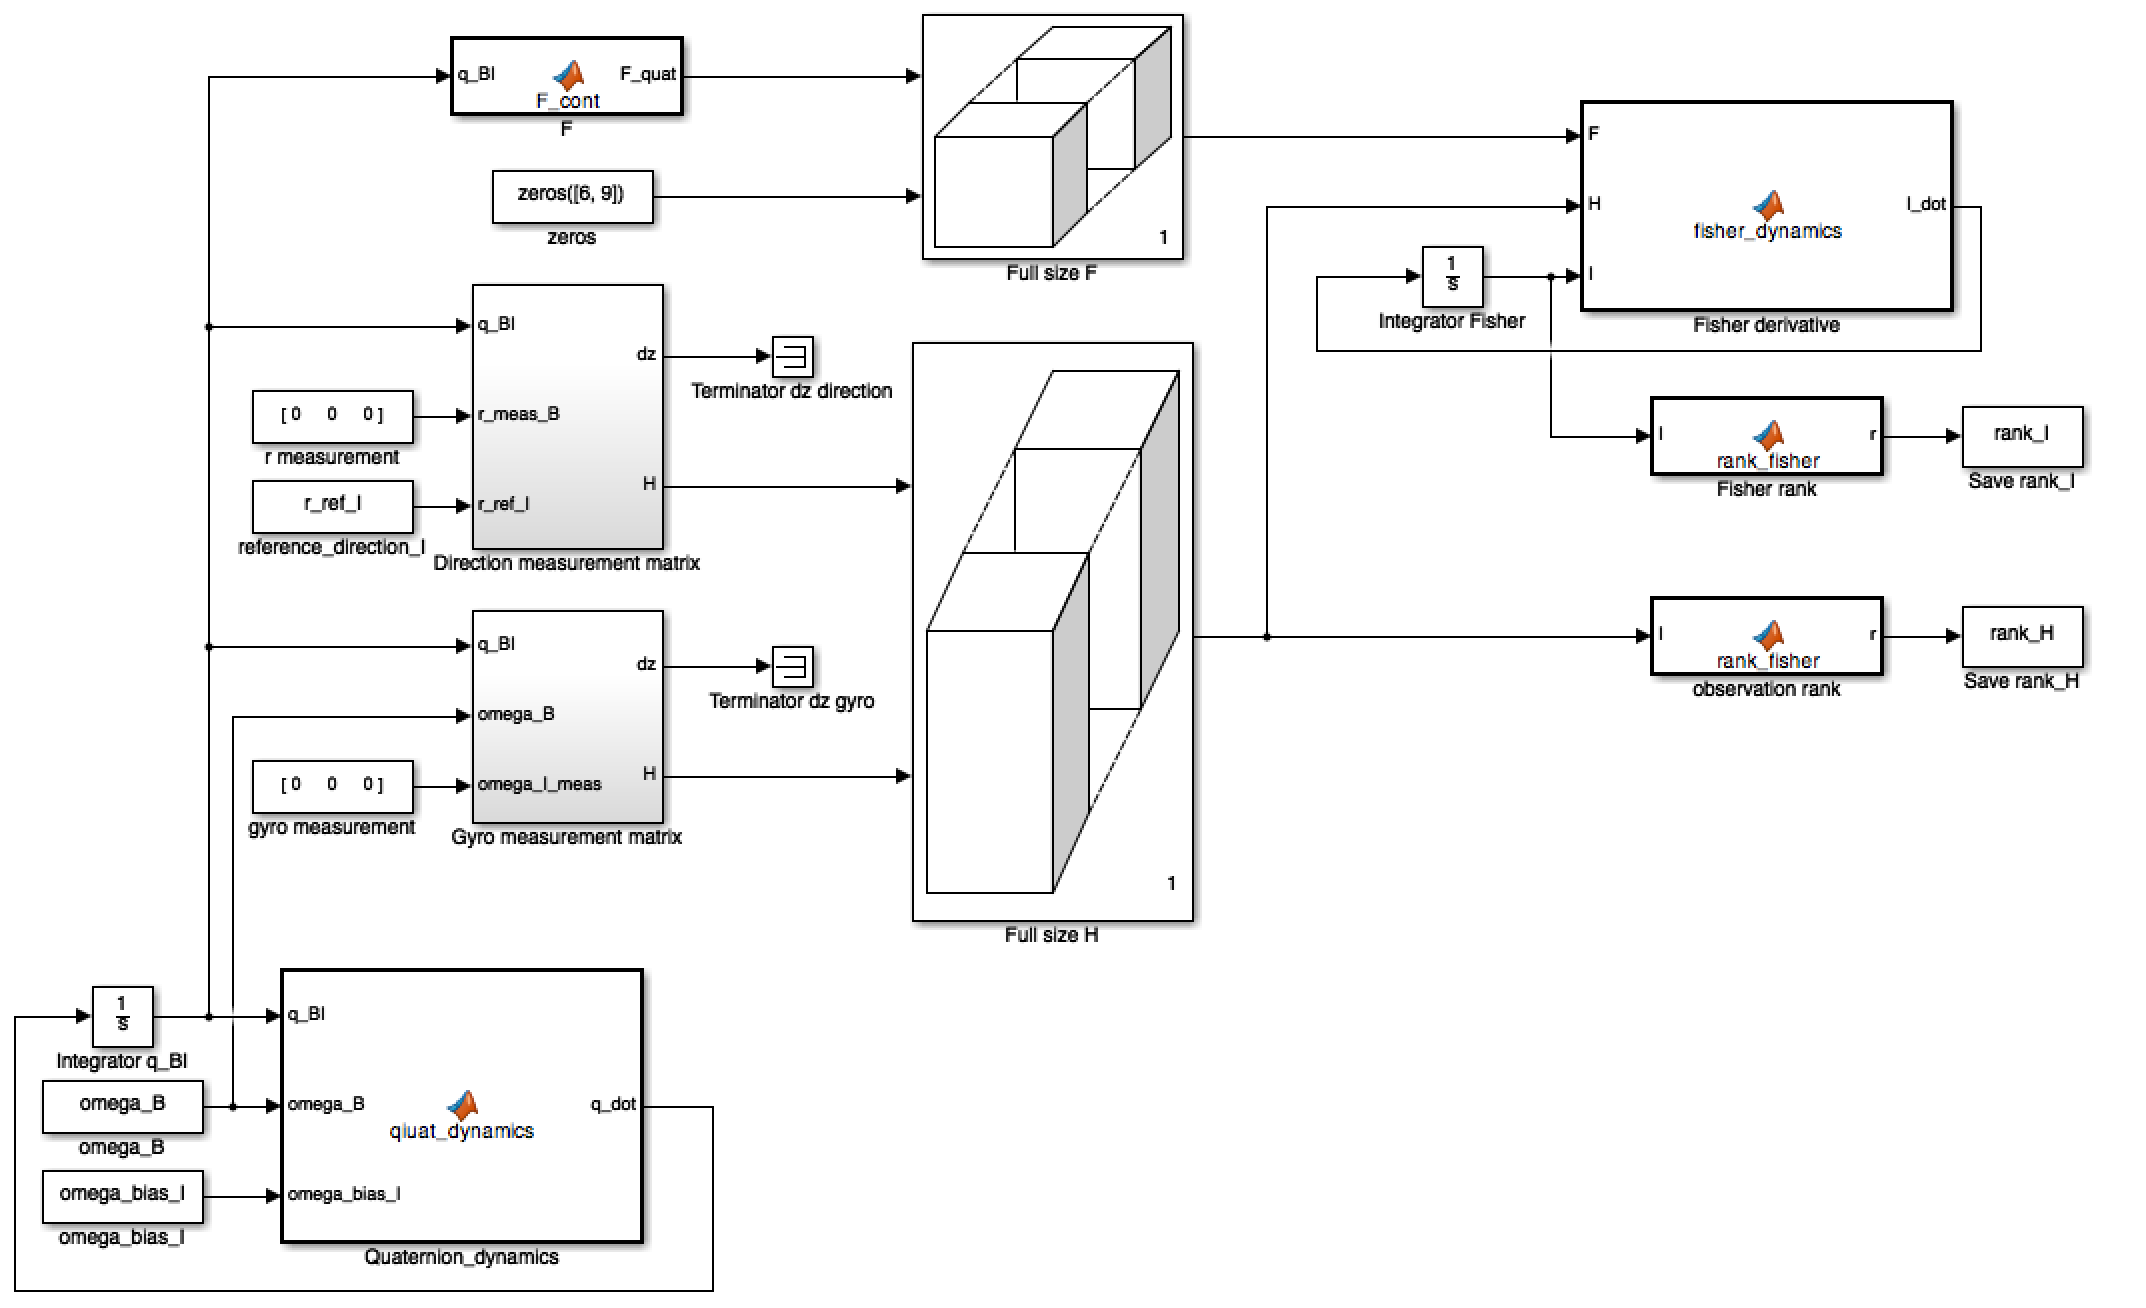
\includegraphics[width=0.8\textwidth]{pic/obs_check.png}
\end{center}
\end{frame}

%--------------------------------------------------------------------------------
\section{Обработка данных с робота}
%--------------------------------------------------------------------------------
\begin{frame}
\frametitle{Модель визуализации оценки на основе реальных данных}
\begin{itemize}
    \item События приходят в порядке возрастания метки времени
    \item События приходят асинхронно
    \item На шаге предиктора необходимо вычислять матрицу
        $\mathbf{Q}\left(\Delta t\right)$ в предположении, что угловое
        ускорение -- это белый шум.
\end{itemize}
\begin{center}
    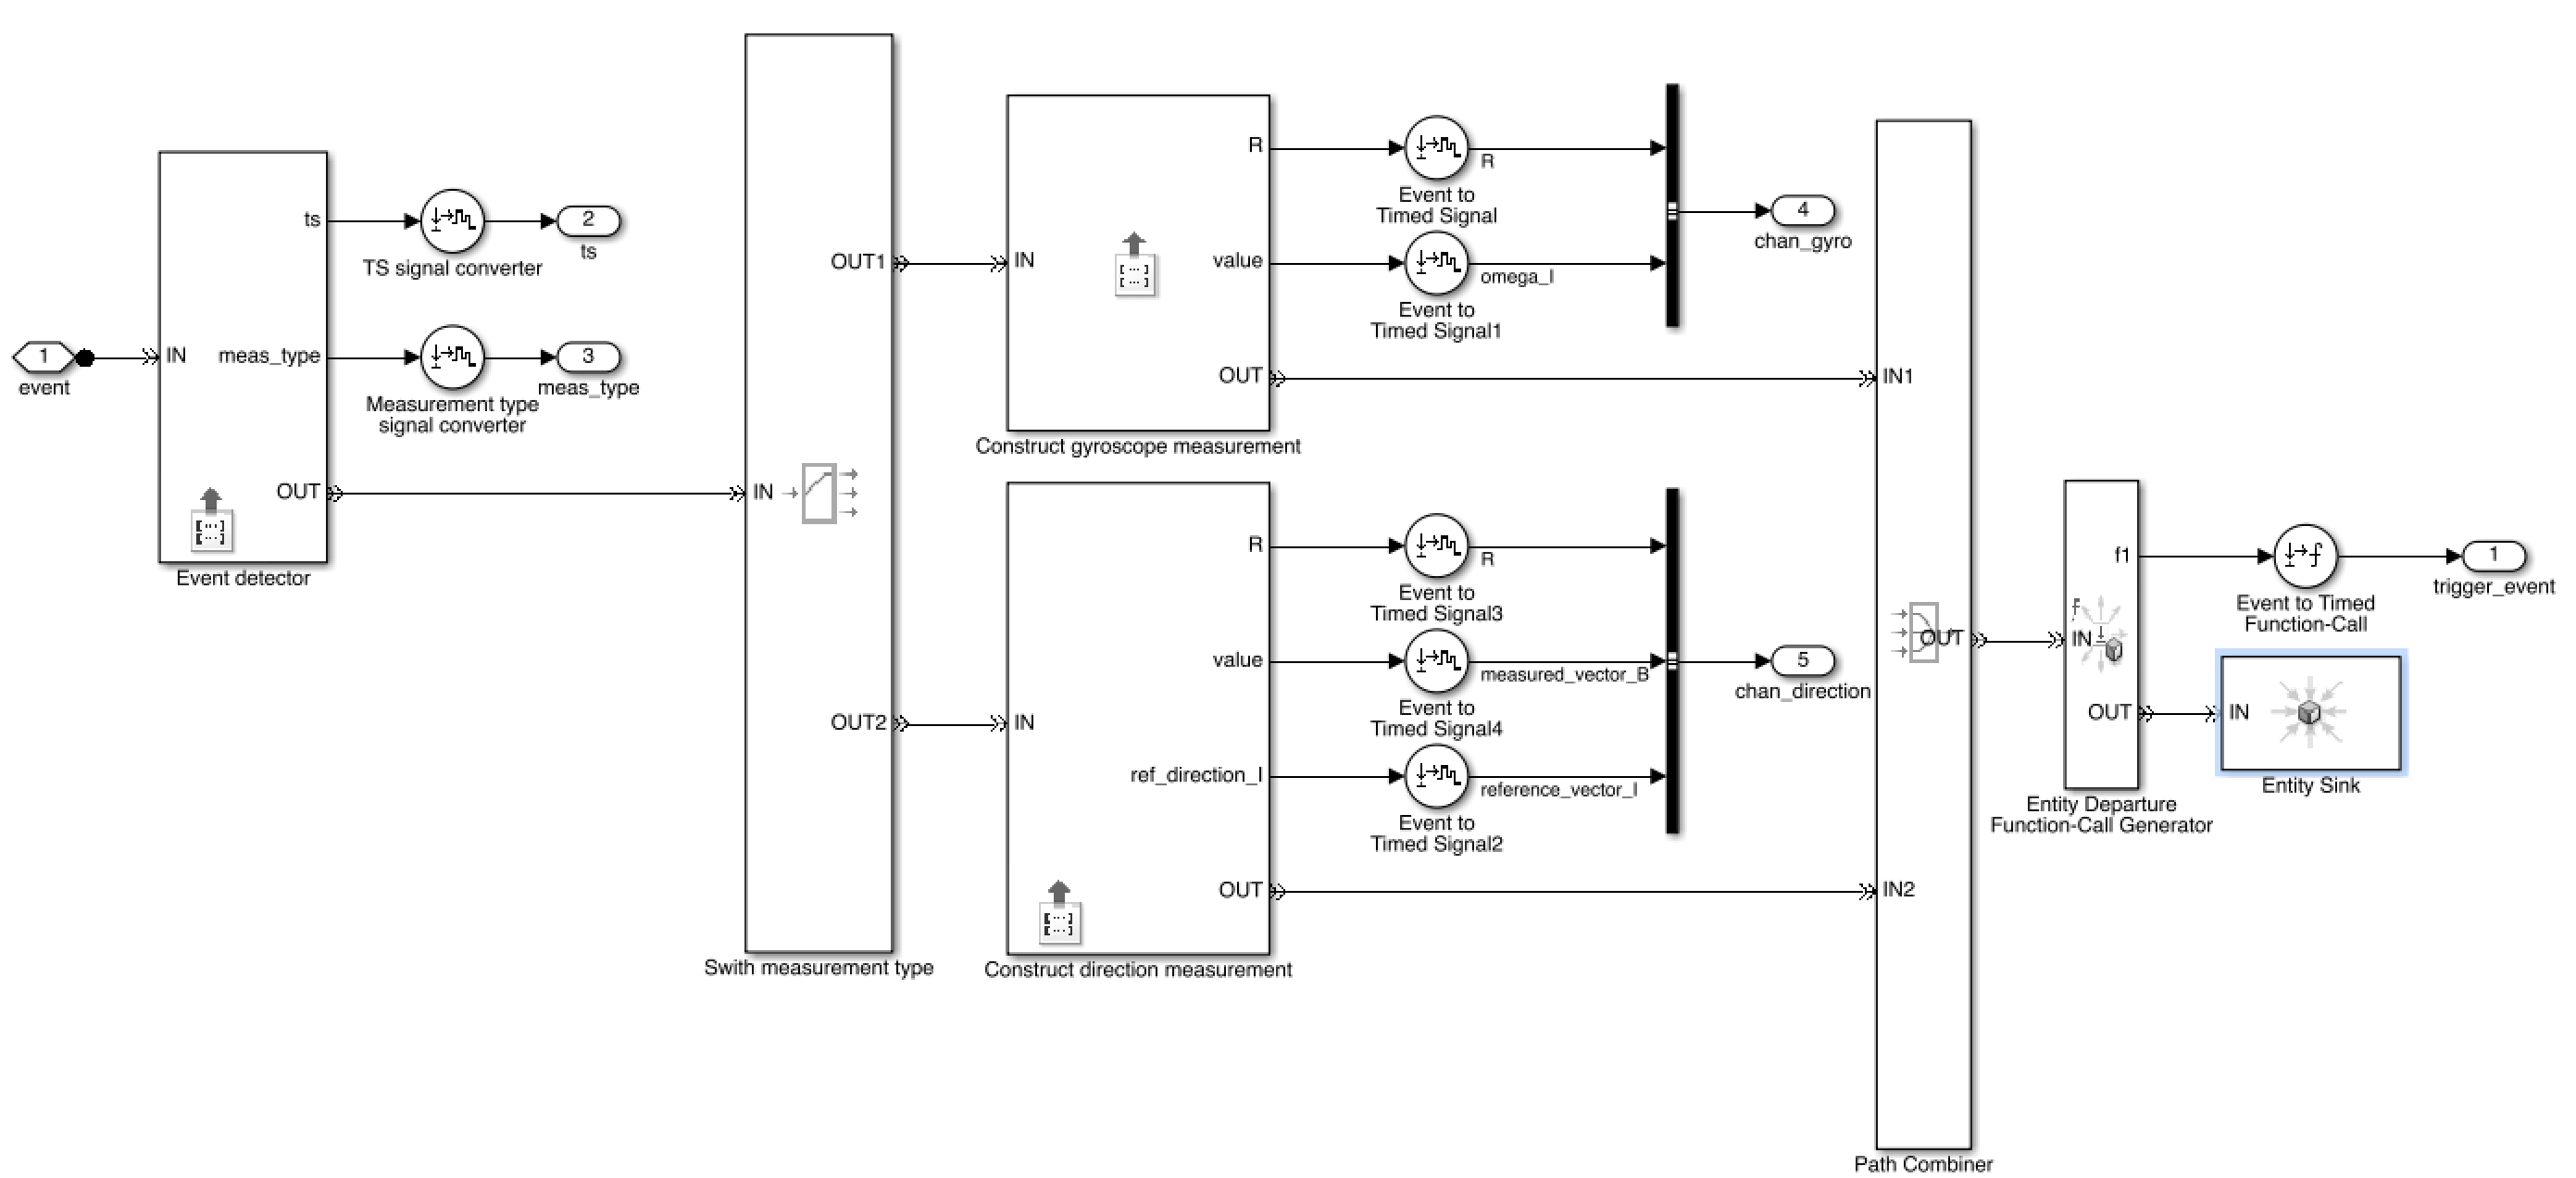
\includegraphics[width=0.8\textwidth]{pic/event_parser.png}
\end{center}
\end{frame}
\begin{frame}
\frametitle{Модель визуализации оценки на основе реальных данных}
\begin{center}
    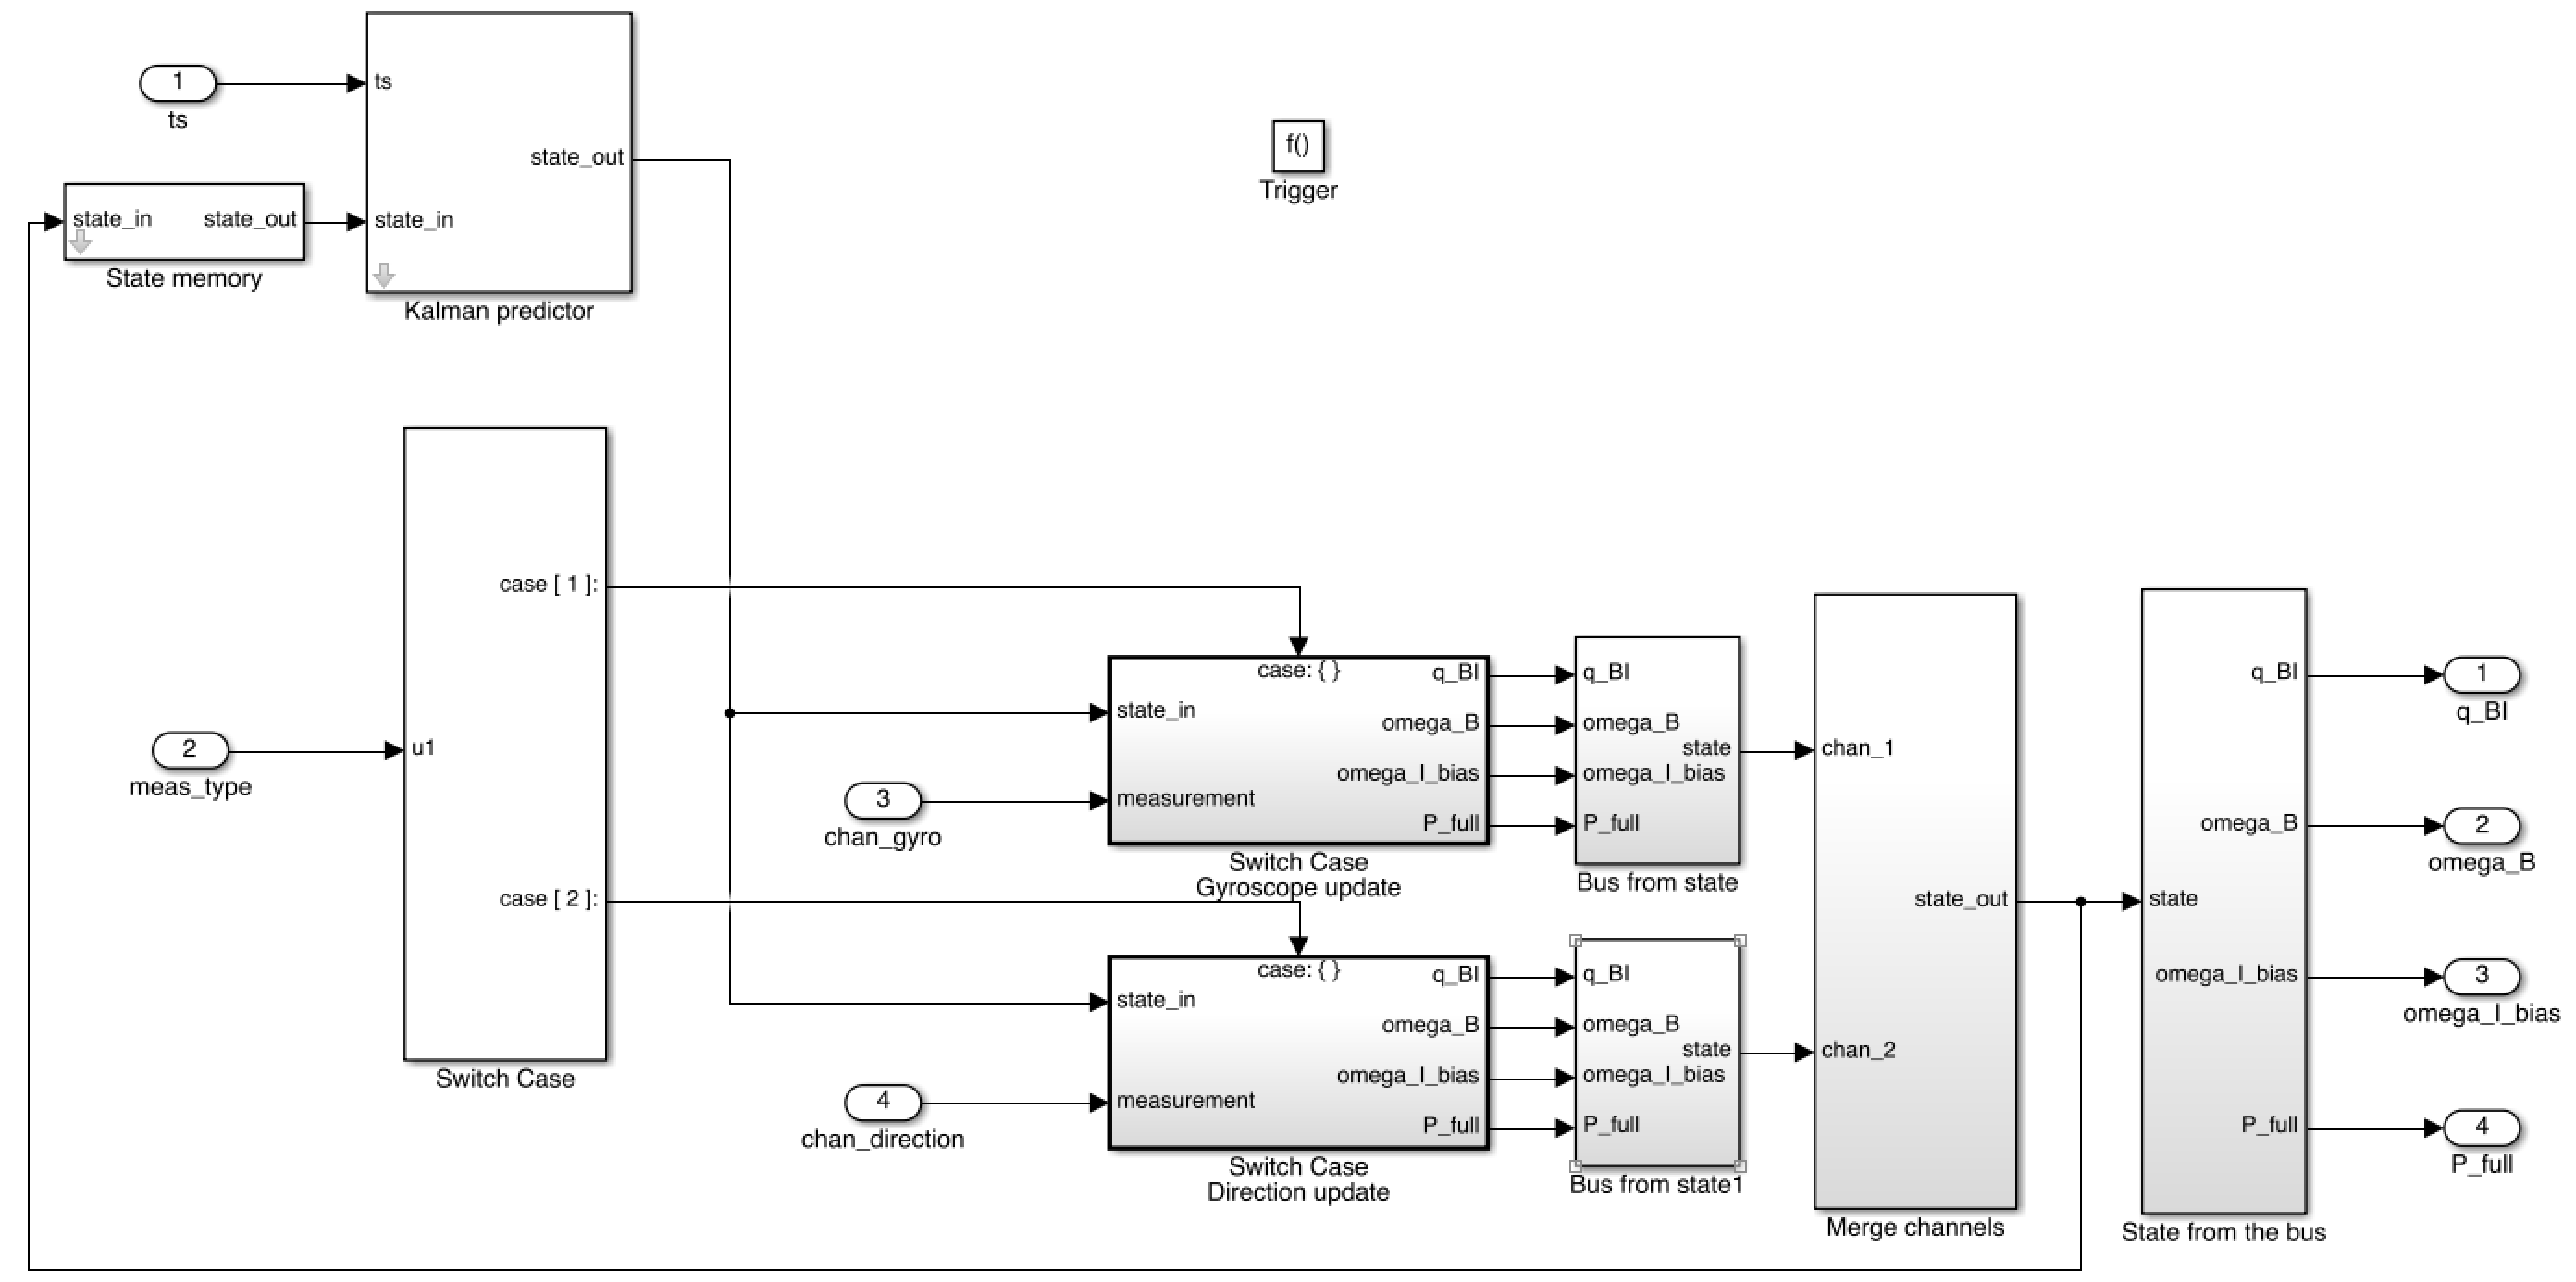
\includegraphics[width=0.8\textwidth]{pic/kalman_triggered.png}
\end{center}
\end{frame}


%--------------------------------------------------------------------------------
\begin{frame}
\frametitle{Заключение}
\begin{itemize}
    \item Получены и валидированы уравнения расширенного фильтра Калмана для
        оценки ориентации и скорости вращения робота в общем трехмерном случае
    \item Показано, что для определения ориентации робота необходимо
        наблюдать за двумя неколлинеарными опорными векторами.
\end{itemize}
\begin{block}{Вопросы для обсуждения}
    \begin{itemize}
        \item Интеграция с визуальной одометрией
        \item Определение скольжения с помощью датчика поворота рулевых колес
        \item Использование вектора поля тяжести в качестве опорного
        \item Использование нескольких акселерометров для оценки угловых
            скоростей
    \end{itemize}
\end{block}
\end{frame}
%--------------------------------------------------------------------------------
\begin{frame}
\frametitle{Литература}
\tiny
\begin{thebibliography}{99}
\bibitem{vectorNav}
{\it Vector NAV laboratory}, \url{http://www.vectornav.com/support/library/gyroscope}
\bibitem{amelkinMIPT}
{\it Н. И. Амелькин}\,
Динамика твердого тела // МФТИ,
\url{https://mipt.ru/education/chair/theoretical_mechanics/upload/a7a/rigid_body-arpgp6n4abs.pdf}

\bibitem{IvanovKeldysh}
    {\it Д. С. Иванов, М. Ю. Овчинников, В. И. Пеньков, Д. С. Ролдугин, Д. М.
Доронин, А. В. Овчинников}, ``Использование магнитных катушек и магнитометра для
обеспечения трехосной ориентации спутника'', Прерпинты ИПМ им. М. В. Келдыша
2015. No 47. 20 с, URL:\url{http://library.keldysh.ru/preprint.asp?id=2015-47}

\bibitem{BarShalom2011}{\it Bar-Shalom Y., Willett P.K. and Tian X. }\, Tracking and Data Fusion: A Handbook of Algorithms. M.: YBS-Press, 2011.
URL: \url{http://books.google.ru/books?id=2aOiuAAACAAJ}.

\bibitem{Technion2009} {\it Technion – Israel Institute of Technology,
    Department of Electrical Engineering} ``Estimation and Identification in
    Dynamical Systems'' (048825)
    Lecture Notes, Fall 2009, Prof. N. Shimkin, \url{http://webee.technion.ac.il/people/shimkin/Estimation09/ch8_target.pdf}

\bibitem{Davis1984}
    M.H.A. Davis, {\it Lectures on stochastic control and nonlinear
    filtering}, Springer Verlag, 1984.

\bibitem{TAC1979}
{\it Taylor, J.H.}, ``The Cramer-Rao estimation error lower bound computation
for deterministic nonlinear systems,'' in Decision and Control including the 17th Symposium on Adaptive Processes, 1978 IEEE Conference on , vol., no., pp.1178-1181, 10-12 Jan. 1979
doi: 10.1109/CDC.1978.268121
\end{thebibliography}
\end{frame}
%--------------------------------------------------------------------------------
\end {document}
